\documentclass[12pt,a4paper,oneside]{report}

\usepackage[a4paper,left=3.2cm,right=2.2cm,top=2.5cm,bottom=2.5cm]{geometry}
\usepackage{fontspec}
\setmainfont{DejaVu Serif}[SmallCapsFont={DejaVu Serif}]
\setsansfont{DejaVu Sans}
\setmonofont{FreeMono}
\usepackage{setspace}
\onehalfspacing
\usepackage{microtype}
\usepackage{amsmath,amssymb,amsthm,mathtools}
\usepackage{booktabs,longtable,tabularx,array,multirow}
\usepackage{enumitem}
\usepackage{xcolor}
\usepackage{listings}
\usepackage{algorithm}
\usepackage[noend]{algpseudocode}
\usepackage{tikz}
\usetikzlibrary{arrows.meta,positioning,calc,shapes.geometric}
\usepackage{pgfplots}
\pgfplotsset{compat=1.18}
\usepackage{graphicx}
\usepackage{caption}
\usepackage{subcaption}
\usepackage[section]{placeins}
\usepackage{fancyhdr}
\usepackage{titlesec}
\usepackage{csquotes}
\usepackage[hidelinks,unicode]{hyperref}
\usepackage[nameinlink,noabbrev]{cleveref}

% Algorithmic line counters restart in each algorithm: keep PDF anchors unique.
\makeatletter
\providecommand{\theHALG@line}{}
\renewcommand{\theHALG@line}{\thealgorithm.\arabic{ALG@line}}
\makeatother

\definecolor{thesisblue}{HTML}{174A7E}
\definecolor{thesisorange}{HTML}{E07B39}
\definecolor{thesisgreen}{HTML}{2D7F5E}
\definecolor{lightgray}{HTML}{F3F5F7}
\hypersetup{
  pdftitle={Đếm đường đi thời gian trên đồ thị có cấu trúc},
  pdfauthor={TÊN SINH VIÊN},
  pdfsubject={Khóa luận tốt nghiệp},
  pdfkeywords={temporal graph, temporal path, series-parallel, treewidth, dynamic programming}
}

\pagestyle{fancy}
\fancyhf{}
\fancyhead[L]{\small\nouppercase{\leftmark}}
\fancyfoot[C]{\thepage}
\renewcommand{\headrulewidth}{0.4pt}
\setlength{\headheight}{15pt}

\renewcommand{\chaptername}{Chương}
\renewcommand{\contentsname}{Mục lục}
\renewcommand{\listfigurename}{Danh mục hình}
\renewcommand{\listtablename}{Danh mục bảng}
\renewcommand{\figurename}{Hình}
\renewcommand{\tablename}{Bảng}
\renewcommand{\bibname}{Tài liệu tham khảo}
\renewcommand{\appendixname}{Phụ lục}
\floatname{algorithm}{Thuật toán}

\titleformat{\chapter}[display]
  {\normalfont\bfseries\color{thesisblue}}
  {\filleft\Large Chương \thechapter}
  {0.5ex}
  {\titlerule\vspace{1ex}\Huge}
\titlespacing*{\chapter}{0pt}{-15pt}{30pt}

\newtheorem{theorem}{Định lý}[chapter]
\newtheorem{lemma}[theorem]{Bổ đề}
\newtheorem{corollary}[theorem]{Hệ quả}
\newtheorem{proposition}[theorem]{Mệnh đề}
\theoremstyle{definition}
\newtheorem{definition}[theorem]{Định nghĩa}
\newtheorem{example}[theorem]{Ví dụ}
\theoremstyle{remark}
\newtheorem{remark}[theorem]{Nhận xét}

\crefname{theorem}{Định lý}{Các định lý}
\crefname{lemma}{Bổ đề}{Các bổ đề}
\crefname{corollary}{Hệ quả}{Các hệ quả}
\crefname{definition}{Định nghĩa}{Các định nghĩa}
\crefname{figure}{Hình}{Các hình}
\crefname{table}{Bảng}{Các bảng}
\crefname{algorithm}{Thuật toán}{Các thuật toán}
\crefname{chapter}{Chương}{Các chương}
\crefname{section}{Mục}{Các mục}

\lstdefinestyle{thesiscode}{
  backgroundcolor=\color{lightgray},
  basicstyle=\ttfamily\small,
  keywordstyle=\color{thesisblue}\bfseries,
  commentstyle=\color{thesisgreen},
  stringstyle=\color{thesisorange},
  numbers=left,
  numberstyle=\tiny\color{gray},
  frame=single,
  breaklines=true,
  columns=fullflexible,
  showstringspaces=false
}
\lstset{style=thesiscode}

\newcommand{\TP}{\textbf{\#Temporal Path}}
\newcommand{\cE}{\mathcal{E}}
\newcommand{\cG}{\mathcal{G}}
\newcommand{\rank}{\operatorname{rank}}
\newcommand{\tw}{\operatorname{tw}}
\newcommand{\bigO}{\mathcal{O}}
\newcommand{\code}[1]{\texttt{#1}}

% ===== THÔNG TIN CẦN THAY TRƯỚC KHI NỘP =====
\newcommand{\UniversityName}{TÊN TRƯỜNG ĐẠI HỌC}
\newcommand{\FacultyName}{KHOA / VIỆN CÔNG NGHỆ THÔNG TIN}
\newcommand{\StudentName}{TÊN SINH VIÊN}
\newcommand{\StudentID}{MÃ SỐ SINH VIÊN}
\newcommand{\SupervisorName}{TÊN GIẢNG VIÊN HƯỚNG DẪN}
\newcommand{\DegreeName}{CỬ NHÂN / KỸ SƯ CÔNG NGHỆ THÔNG TIN}
\newcommand{\ThesisYear}{2026}

\setlength{\emergencystretch}{2em}
% Automatically generated; do not edit values by hand.
\newcommand{\AuditComparisons}{741\,280}
\newcommand{\AuditQueryModes}{259\,856}
\newcommand{\AtlasGraphs}{495}
\newcommand{\BenchCases}{190}
\newcommand{\BenchSuccessfulSamples}{3\,290}
\newcommand{\BenchTimeouts}{15}
\newcommand{\BenchSkips}{3}
\newcommand{\TTSPMatrixTime}{365}
\newcommand{\TTSPEventTime}{7.53}
\newcommand{\TTSPSpeedup}{48.4}
\newcommand{\TTSPMatrixRSS}{92.6}
\newcommand{\TTSPEventRSS}{8.01}
\newcommand{\ForestPairedCells}{47}
\newcommand{\ForestCensoredCells}{2}
\newcommand{\ForestGeoSpeedup}{16.1}
\newcommand{\DPGeoSpeedup}{3.8}
\newcommand{\CactusGeoSpeedup}{78.9}
\newcommand{\AblationCombinedSpeedup}{5.93}


\begin{document}
\pagenumbering{gobble}
\begin{titlepage}
\begin{center}
{\large\bfseries \UniversityName\\[0.4cm] \FacultyName}

\vfill

{\Large\bfseries KHÓA LUẬN TỐT NGHIỆP\\[0.8cm]}
{\fontsize{20}{26}\selectfont\bfseries\color{thesisblue}
ĐẾM ĐƯỜNG ĐI THỜI GIAN TRÊN RỪNG,\\
ĐỒ THỊ SERIES--PARALLEL VÀ\\
ĐỒ THỊ CÓ TREEWIDTH BỊ CHẶN}

\vfill

\begin{tabular}{rl}
Sinh viên thực hiện: & \textbf{\StudentName} \\
Mã số sinh viên: & \StudentID \\
Giảng viên hướng dẫn: & \textbf{\SupervisorName} \\
Chương trình: & \DegreeName
\end{tabular}

\vfill

{\large Thành phố Hồ Chí Minh, \ThesisYear}
\end{center}
\end{titlepage}


\clearpage
\pagenumbering{roman}
\chapter*{Lời cam đoan}
\addcontentsline{toc}{chapter}{Lời cam đoan}

Tôi cam đoan khóa luận này trình bày trung thực quá trình nghiên cứu, thiết kế thuật toán, cài đặt và thực nghiệm của tôi dưới sự hướng dẫn của giảng viên hướng dẫn. Các kết quả từ công trình của tác giả khác đều được ghi nguồn. Phần mềm, tập sinh dữ liệu và kịch bản thực nghiệm đi kèm khóa luận cho phép tái lập các kết quả được báo cáo.

Kết quả về đồ thị series--parallel và treewidth trong khóa luận là kết quả nghiên cứu đang chờ thẩm định độc lập; khóa luận không tuyên bố kết quả này đã qua bình duyệt. Các số liệu thực nghiệm được mô tả đúng phạm vi đã chạy và không được gọi là bộ benchmark chính thức của bài báo gốc.

\vspace{2cm}
\begin{flushright}
\StudentName\\
Ngày \dotfill tháng \dotfill năm \ThesisYear
\end{flushright}


\chapter*{Lời cảm ơn}
\addcontentsline{toc}{chapter}{Lời cảm ơn}

Tôi xin gửi lời cảm ơn chân thành đến \SupervisorName{} vì sự hướng dẫn, phản biện và hỗ trợ trong suốt quá trình thực hiện khóa luận. Tôi cảm ơn các thầy cô tại \FacultyName{} đã cung cấp nền tảng về thuật toán, lý thuyết đồ thị và phương pháp nghiên cứu khoa học. Tôi cũng cảm ơn gia đình và bạn bè đã động viên trong quá trình xây dựng chứng minh, cài đặt phần mềm và thực hiện các chiến dịch kiểm thử.

Khóa luận kế thừa câu hỏi mở được Enright, Meeks và Molter nêu trong công trình \emph{Counting Temporal Paths}. Tôi trân trọng giá trị của công trình này trong việc định hình bài toán, thuật ngữ và bối cảnh độ phức tạp cho nghiên cứu hiện tại.


\chapter*{Tóm tắt}
\addcontentsline{toc}{chapter}{Tóm tắt}

Khóa luận nghiên cứu đếm chính xác đường đi thời gian đơn giữa hai đỉnh trong đồ thị vô hướng, tập trung vào rừng, two-terminal series--parallel, cactus và đồ thị có treewidth bị chặn. Công trình \emph{Counting Temporal Paths} của Enright, Meeks và Molter đưa ra truy hồi $\bigO(|V|T^2)$ trên rừng, FPT theo tổ hợp treewidth và lifetime, và giả thuyết mở rộng đa thức sang series--parallel. Khóa luận phát triển các thuật toán tường minh cho khoảng trống này, phân biệt số phép toán số học với chi phí bit và tiền xử lý.

Trên rừng, tổng tiền tố giảm đánh giá truy hồi xuống $\bigO(|P|r)$; bản thưa đạt $\bigO(|P|+M_P)$ phép toán sau khi có đường và nhãn đã sắp. Với TTSP có hai cực là truy vấn, khóa luận trình bày ma trận truyền $\bigO(mr^3)$ rồi thay bằng định hướng DAG và quét sự kiện. Lõi mới dùng $\bigO(n+m+M+r)$ thao tác và đúng $M$ phép cộng số đếm, không cần nhân số đếm. Phân rã block--cut mở rộng phương pháp sang cactus với terminal tùy ý.

Đối với treewidth $w$, DP giữ bậc có hướng, nhãn cục bộ và phân hoạch liên thông; tính acyclic tại join được chứng minh bằng đẳng thức hạng chu trình của hợp hai rừng và incidence multigraph. Xóa nhãn terminal giảm cận trạng thái theo $r$ từ bậc $w+3$ xuống $w+1$, cho thời gian
\[
 N(r+1)^{2w+2}2^{\bigO(w\log w)}.
\]
Với $w=2$, cận an toàn là $\bigO(N(r+1)^6)$, suy ra thuật toán đa thức trên series--parallel với đầu cuối tùy ý. Đây là XP theo treewidth, không phải FPT chỉ theo treewidth. Cả strict và non-strict được chứng minh và kiểm thử riêng trên các lớp này.

Hiện thực C++20 dùng số nguyên chính xác độ dài tùy ý. Chiến dịch mới có \AuditComparisons{} đối chiếu không sai lệch, gồm vét cạn $n\le4,r=2$, $n=5,r=1$, \AtlasGraphs{} Graph Atlas width không quá hai, dữ liệu random width 1--4 và metamorphic tests. Benchmark có \BenchCases{} cấu hình, bảy lần đo cho mỗi solver hoàn thành, median/IQR, CPU time của solver và RSS sau exec. Trên các cell cùng hoàn thành, dense forest nhanh hơn truy hồi gốc trung bình nhân \ForestGeoSpeedup{} lần; DP compact nhanh hơn bản trước \DPGeoSpeedup{} lần trên partial 2-tree. TTSP 256 diamond tại $r=32$ đạt tỷ số \TTSPSpeedup{} lần so với ma trận. Ladder 64 cột có $2^{63}$ tuyến tĩnh vẫn được DP đếm đúng theo oracle đóng.

Các định lý là kết quả được trình bày và kiểm chứng trong bản thảo; tuyên bố tính mới quốc tế vẫn cần thẩm định độc lập. Khóa luận không gọi chiến dịch hiện tại là vét cạn $n=5,r=2$, không so tốc độ với mã MSO tác giả chưa có, và không suy rộng synthetic benchmarks sang mọi mạng thực.

\noindent\textbf{Từ khóa:} đồ thị thời gian; đếm chính xác; series--parallel; cactus; treewidth; strict paths; quy hoạch động; thực nghiệm tái lập.

\chapter*{Abstract}
\addcontentsline{toc}{chapter}{Abstract}

This thesis develops explicit exact algorithms for simple temporal paths in undirected structured graphs. It improves the forest recurrence from quadratic to linear rank dependence, and obtains sparse-label counting proportional to relevant label incidences. For pole-to-pole TTSP queries, a proved acyclic orientation enables an event counter performing exactly one count addition per temporal edge after preprocessing, replacing the internal cubic-rank transfer-matrix baseline. A block-cut route extends the event method to arbitrary-terminal cactus queries.

A connectivity dynamic program on a supplied width-$w$ tree decomposition uses local time inequalities and a cycle-rank proof at joins. Erasing terminal timestamps reduces the rank exponent of the state bound by two and yields $N(r+1)^{2w+2}2^{\bigO(w\log w)}$ arithmetic operations. The width-two specialization gives $\bigO(N(r+1)^6)$ and a proposed polynomial solution for arbitrary-terminal series--parallel graphs. Both strict and non-strict variants are proved and implemented; the parameter classification remains XP rather than treewidth-only FPT.

A C++20 implementation with arbitrary-precision integers passes \AuditComparisons{} solver/oracle comparisons. The \BenchCases{}-cell campaign reports repeated median/IQR measurements, proper child-process CPU time, post-exec peak RSS and censored cases. Dense forest and optimized partial-two-tree DP obtain geometric-mean speedups of \ForestGeoSpeedup{} and \DPGeoSpeedup{} on paired completed cells. A 64-column ladder with $2^{63}$ static routes is counted exactly using an independent closed-form oracle. Worldwide novelty and final proof acceptance remain subject to independent academic review.


\tableofcontents
\clearpage
\listoffigures
\clearpage
\listoftables
\clearpage
\chapter*{Danh mục ký hiệu và chữ viết tắt}
\addcontentsline{toc}{chapter}{Danh mục ký hiệu và chữ viết tắt}

\begin{longtable}{>{\bfseries}p{3.2cm}p{10.2cm}}
$V,E$ & Tập đỉnh và tập cạnh của đồ thị nền tĩnh.\\
$\cE$ & Tập cạnh--thời gian $(e,t)$.\\
$T$ & Lifetime, tức nhãn thời gian lớn nhất trong biểu diễn gốc.\\
$r$ & Số giá trị thời gian phân biệt sau nén hạng.\\
$L(e)$ & Danh sách hạng thời gian hoạt động của cạnh tĩnh $e$.\\
$s,z$ & Đỉnh nguồn và đỉnh đích của truy vấn.\\
$N$ & Đại lượng kích thước đầu vào $|V|+|\cE|$.\\
$w$ & Treewidth của đồ thị nền.\\
TTSP & Two-terminal series--parallel.\\
TD & Tree decomposition, phân rã cây.\\
MSO & Monadic second-order logic.\\
FPT & Fixed-parameter tractable.\\
XP & Lớp bài toán có thời gian $N^{f(k)}$ theo tham số $k$.\\
DP & Dynamic programming, quy hoạch động.\\
RSS & Resident set size, bộ nhớ vật lý cực đại được báo cáo.\\
\end{longtable}


\clearpage
\pagenumbering{arabic}
\chapter{Giới thiệu}
\label{chap:introduction}

\section{Bối cảnh và động lực}

Nhiều mạng thực tế không bất biến theo thời gian. Liên kết giữa hai người chỉ tồn tại khi họ gặp nhau; một chuyến xe chỉ nối hai địa điểm tại một thời điểm cụ thể; một liên kết truyền thông chỉ khả dụng trong một khoảng thời gian. Mô hình đồ thị tĩnh làm mất thứ tự của các tương tác và có thể kết luận sai rằng một hành trình tồn tại dù các cạnh của hành trình xuất hiện theo thứ tự không khả thi. Đồ thị thời gian khắc phục vấn đề này bằng cách gắn thời điểm hoạt động cho mỗi cạnh.

Một đường đi thời gian không chỉ phải là đường đi trong đồ thị nền mà còn phải tôn trọng thứ tự thời gian. Việc tìm một đường đi như vậy thường dễ hơn đáng kể so với việc đếm tất cả đường đi. Số lượng đường đi liên quan trực tiếp tới độ dư thừa của kết nối, phân tích độ tin cậy và các đại lượng trung tâm dựa trên đường đi. Công trình \emph{Counting Temporal Paths} của Enright, Meeks và Molter khởi đầu nghiên cứu có hệ thống về độ phức tạp tham số và xấp xỉ của bài toán này \cite{enright2025}.

Bài báo chứng minh bài toán khó ngay cả dưới những hạn chế cấu trúc mạnh, nhưng cũng chỉ ra một số miền khả giải. Đặc biệt, khi đồ thị nền là rừng, đường đi tĩnh giữa hai đỉnh là duy nhất và một truy hồi theo thời gian cho thuật toán $\bigO(|V|T^2)$. Khi tham số hóa đồng thời bởi treewidth và lifetime, bài toán là FPT nhờ một biểu diễn MSO và định lý Courcelle. Trong phần kết luận, các tác giả dự đoán rằng thuật toán đa thức trên rừng có thể mở rộng sang đồ thị series--parallel \cite{enright2025}.

Câu hỏi này hấp dẫn vì series--parallel là lớp đầu tiên vượt ra ngoài rừng nhưng vẫn có cấu trúc phân rã chặt. Ghép song song tạo ra nhiều tuyến tĩnh, thậm chí số tuyến tăng theo hàm mũ trong kích thước biểu diễn. Vì vậy, liệt kê đường đi không còn là một chiến lược đa thức. Đồng thời, treewidth của lớp này không quá $2$, gợi ý rằng một trạng thái cục bộ đủ giàu có thể nén được toàn bộ lịch sử đường đi.

\section{Phát biểu vấn đề}

Cho đồ thị thời gian vô hướng $\cG=(V,\cE,T)$ và hai đỉnh phân biệt $s,z\in V$. Mỗi phần tử của $\cE$ có dạng $(\{u,v\},t)$ với $t\in[T]$. Một đường đi thời gian không nghiêm ngặt là một đường đi tĩnh đơn
\[
  P=(v_0=s,v_1,\ldots,v_\ell=z)
\]
cùng lựa chọn thời điểm $t_i\in L(\{v_{i-1},v_i\})$ sao cho
\[
  t_1\le t_2\le\cdots\le t_\ell.
\]
Bài toán \TP{} yêu cầu đếm chính xác tất cả các đối tượng như vậy. Hai lựa chọn nhãn thời gian khác nhau trên cùng đường đi tĩnh được tính là hai đường đi thời gian khác nhau.

Khóa luận tập trung vào bốn câu hỏi nghiên cứu:

\begin{description}[leftmargin=2.2cm,style=nextline]
  \item[RQ1.] Có thể đánh giá truy hồi trên rừng nhanh hơn cận $\bigO(|V|T^2)$ đã công bố hay không?
  \item[RQ2.] Có thể đếm TTSP cực--cực theo số nhãn thực sự mà không dựng toàn bộ ma trận truyền hay liệt kê số tuyến hàm mũ hay không?
  \item[RQ3.] Có thể đưa ra thuật toán tường minh tham số hóa chỉ bởi treewidth của đồ thị nền, thay cho meta-algorithm phụ thuộc đồng thời vào lifetime hay không?
  \item[RQ4.] Cài đặt thực tế có đồng ý với các oracle khép kín và phương pháp brute force độc lập hay không, và xu hướng thời gian chạy có phù hợp với phân tích hay không?
\end{description}

\section{Đóng góp}

Khóa luận đưa ra các đóng góp sau.

\begin{enumerate}[label=\textbf{C\arabic*.}]
  \item Chứng minh nén hạng thời gian bảo toàn song ánh tập đường đi thời gian. Trên rừng, sử dụng tổng tiền tố để giảm thời gian xuống $\bigO(|P|r)$ và sử dụng hai con trỏ trên danh sách thưa để đạt
  \[
    \bigO\!\left(|P|+\sum_{e\in P}|L(e)|\right).
  \]
  \item Xây dựng ma trận truyền TTSP làm baseline $\bigO(mr^3)$, sau đó chứng minh song ánh với đường đi trong DAG định hướng chuẩn và đưa ra lõi quét sự kiện $\bigO(n+m+M+r)$, gồm đúng $M$ phép cộng số đếm sau nén hạng và định hướng. Với $M=|\cE|$, bộ nhớ không cần ma trận $r\times r$ ở mọi nút.
  \item Mở rộng quét sự kiện sang cactus với đầu cuối tùy ý bằng route block--cut; các block ngoài route bị loại đúng theo tính đơn của đường đi.
  \item Xây dựng quy hoạch động kết nối trên nice tree decomposition. Trạng thái ghi bậc có hướng kèm thời điểm cục bộ và phân hoạch liên thông. Một kiểm tra đồ thị incidence hai phía tại nút join ngăn chu trình, kể cả chu trình độ dài hai do cạnh song song trong incidence multigraph.
  \item Chứng minh thuật toán treewidth chạy trong
  \[
    N(r+1)^{2w+2}2^{\bigO(w\log w)}
  \]
  phép toán số học sau xóa nhãn terminal; cận trạng thái giảm từ bậc $w+3$ xuống $w+1$ theo $r$. Với $w=2$, cận an toàn là $\bigO(N(r+1)^6)$, vẫn là XP chứ không phải FPT chỉ theo treewidth.
  \item Chứng minh và cài đặt cả biến thể non-strict/strict trên các lớp đang xét. Cung cấp C++20 số nguyên độ dài tùy ý, oracle Python liệt kê cạnh thời gian, kiểm thử vét cạn và Graph Atlas. Chiến dịch mới có \AuditComparisons{} đối chiếu không sai lệch; benchmark có \BenchCases{} cấu hình, bảy lần đo và hình/bảng sinh tự động từ CSV.
\end{enumerate}

\section{Phạm vi và mức độ khẳng định}

Khóa luận xét đồ thị thời gian vô hướng, đường đi đơn, và cả hai điều kiện $\le$/$<$. Không xét temporal walks, thời gian chờ bị chặn hoặc độ trễ di chuyển dương. Thuật toán tổng quát nhận một phân rã cây hợp lệ; riêng width không quá $2$ có bộ nhận dạng và sinh phân rã bằng elimination. Chi phí đọc/nén input, xác nhận cấu trúc và số học nhiều bit được tách rõ khỏi cận lõi đếm.

Kết quả series--parallel là đóng góp nghiên cứu của khóa luận, không phải kết quả từ bài báo 2025. Bằng chứng thực nghiệm không thay thế chứng minh, và chứng minh nội bộ không thay thế bình duyệt. Do đó, cách diễn đạt an toàn là: khóa luận \emph{đề xuất và cài đặt} một lời giải đa thức cho trường hợp series--parallel, giải giả thuyết đã nêu \emph{với điều kiện} kết quả vượt qua thẩm định độc lập và kiểm tra tính mới.

\section{Cấu trúc khóa luận}

\Cref{chap:background} trình bày nền tảng và công trình liên quan. \Cref{chap:forests} phát triển hai cải tiến trên rừng. \Cref{chap:ttsp} đưa ra đại số truyền TTSP. \Cref{chap:treewidth} trình bày thuật toán treewidth, chứng minh đúng và hệ quả series--parallel. \Cref{chap:implementation} mô tả cài đặt và khả năng tái lập. \Cref{chap:experiments} trình bày thực nghiệm và đe dọa tới tính hợp lệ. Cuối cùng, \Cref{chap:conclusion} tổng kết câu trả lời cho các câu hỏi nghiên cứu và hướng phát triển.

\chapter{Cơ sở lý thuyết và công trình liên quan}
\label{chap:background}

\section{Đồ thị thời gian}

\begin{definition}[Đồ thị thời gian]
Một đồ thị thời gian vô hướng, đơn là bộ ba $\cG=(V,\cE,T)$, trong đó $V$ là tập đỉnh, $T\in\mathbb{N}$ là lifetime và
\[
  \cE\subseteq \binom{V}{2}\times[T]
\]
là tập cạnh--thời gian. Đồ thị nền $G=(V,E)$ chứa cạnh $e$ khi tồn tại ít nhất một $t$ sao cho $(e,t)\in\cE$.
\end{definition}

Với cạnh tĩnh $e$, ký hiệu $L(e)=\{t:(e,t)\in\cE\}$. Một đường đi thời gian phải đơn về đỉnh ở lớp tĩnh; do đó, nó khác với temporal walk, nơi một đỉnh có thể xuất hiện nhiều lần. Khóa luận lấy quy ước không nghiêm ngặt của Enright và cộng sự làm thiết lập chính, đồng thời kiểm chứng riêng biến thể nghiêm ngặt. Các nhãn liên tiếp lần lượt thỏa $\le$ và $<$ \cite{enright2025}. Thứ tự sự kiện bằng thời điểm là quan trọng trong cả chứng minh và kiểm thử.

\begin{example}
Xét đường đi tĩnh $s-u-z$ với $L(su)=\{1,2\}$ và $L(uz)=\{2,3\}$. Bốn lựa chọn hợp lệ là $(1,2),(1,3),(2,2),(2,3)$. Nếu dùng định nghĩa nghiêm ngặt, lựa chọn $(2,2)$ bị loại và đáp án còn ba.
\end{example}

\section{Đếm chính xác và độ phức tạp tham số}

Giá trị đếm có thể lớn theo hàm mũ, nên thời gian chạy cần được hiểu theo cả số phép toán số học và độ dài bit. Với mỗi cạnh tĩnh, một nghiệm cục bộ có tối đa $1+2r$ lựa chọn gồm bỏ qua hoặc chọn một trong hai hướng và một hạng thời gian. Một cận thô cho giá trị trung gian là $(1+2r)^{|E|}$, tương ứng $\bigO(|E|\log(1+2r))$ bit, kể cả $r=1$. Vì vậy, với treewidth cố định, chi phí bit của số nguyên lớn vẫn là đa thức.

Một bài toán tham số hóa bởi $k$ thuộc FPT nếu giải được trong $f(k)N^{\bigO(1)}$; nó thuộc XP nếu thời gian là $N^{f(k)}$. Khác biệt này có ý nghĩa ở đây. Bài báo gốc cho FPT theo \emph{tổ hợp} treewidth và lifetime bằng MSO/Courcelle \cite{enright2025,courcelle2012}. Thuật toán của khóa luận bỏ lifetime khỏi tập tham số nhưng đạt XP, không phải FPT, theo treewidth. Điều này không mâu thuẫn với kết quả hardness theo feedback vertex number trong bài báo gốc.

\section{Nén hạng thời gian}

Giả sử các nhãn thực sự xuất hiện là
\[
  \tau_1<\tau_2<\cdots<\tau_r.
\]
Thay $\tau_i$ bởi $i$.

\begin{lemma}[Bảo toàn qua nén hạng]
Phép nén hạng tạo song ánh giữa các đường đi thời gian trước và sau biến đổi.
\end{lemma}

\begin{proof}
Tính khả thi chỉ dùng các so sánh $t_i\le t_{i+1}$. Ánh xạ hạng bảo toàn thứ tự chặt, nên
\[
  \tau_i\le\tau_j \iff i\le j.
\]
Đường đi tĩnh và lựa chọn lần xuất hiện của mỗi cạnh không thay đổi. Ánh xạ thuận và nghịch do đó bảo toàn từng nghiệm.
\end{proof}

Hệ quả thực hành là độ phức tạp nên viết theo $r$ thay vì giá trị số lớn nhất $T$. Luôn có $r\le|\cE|$, kể cả khi timestamp gốc là Unix time hoặc số nguyên rất thưa.

\section{Rừng, series--parallel và treewidth}

Trong rừng, giữa $s$ và $z$ có nhiều nhất một đường đi tĩnh. Điều này loại bỏ phần khó về lựa chọn topology và chỉ còn đếm chuỗi nhãn không giảm.

Đồ thị TTSP được xây dựng đệ quy từ một cạnh có thứ tự hai cực $(x,y)$ bằng hai phép:
\begin{itemize}
  \item \emph{series}: đồng nhất cực phải của thành phần thứ nhất với cực trái của thành phần thứ hai;
  \item \emph{parallel}: đồng nhất đồng thời hai cặp cực tương ứng.
\end{itemize}
Khái niệm series--parallel trong tài liệu có một số biến thể. Khóa luận phân biệt thuật toán TTSP chuyên biệt, yêu cầu truy vấn trùng hai cực, với hệ quả treewidth áp dụng cho partial $2$-tree và đầu cuối tùy ý. Việc nhận dạng và phân rã series--parallel có thể thực hiện hiệu quả \cite{eppstein1992}.

\begin{definition}[Phân rã cây]
Một phân rã cây của $G=(V,E)$ là cây $\mathcal{T}$ với mỗi nút $x$ mang bag $B_x\subseteq V$, thỏa:
\begin{enumerate}
  \item mỗi đỉnh xuất hiện trong ít nhất một bag;
  \item với mọi $uv\in E$, có bag chứa cả $u,v$;
  \item các bag chứa một đỉnh cố định tạo thành cây con liên thông.
\end{enumerate}
Độ rộng là $\max_x|B_x|-1$; treewidth $\tw(G)$ là độ rộng nhỏ nhất.
\end{definition}

Nice tree decomposition dùng các nút leaf, introduce-vertex, introduce-edge, forget-vertex và join. Trong khóa luận, $s,z$ được thêm vào mọi bag; nếu phân rã ban đầu có độ rộng $w$, kích thước bag sau chuẩn hóa không quá $w+3$. Mỗi cạnh tĩnh được introduce đúng một lần.

\section{Kết quả đã biết và khoảng trống nghiên cứu}

Bài báo Algorithmica 2025 chứng minh ba dữ kiện định hướng nghiên cứu này \cite{enright2025}:
\begin{enumerate}
  \item \TP{} khó trong trường hợp tổng quát và có hardness tham số mạnh;
  \item trường hợp đồ thị nền là rừng giải được trong $\bigO(|V|T^2)$;
  \item trường hợp tham số hóa đồng thời bởi treewidth và lifetime là FPT nhờ MSO.
\end{enumerate}
Bài báo kết thúc bằng giả thuyết rằng thuật toán trên rừng mở rộng được sang series--parallel, gợi ý khai thác phép ghép song song. Phiên bản STACS 2023 cung cấp bản tóm lược sớm hơn của hướng nghiên cứu \cite{enright2023}.

Khoảng trống có hai tầng. Ở tầng kỹ thuật, chưa có thuật toán thực thi cho series--parallel hoặc DP treewidth tường minh trong công trình gốc. Ở tầng thực nghiệm, bài báo mang tính lý thuyết và không cung cấp bộ benchmark hay mã nguồn tác giả. Vì vậy, khóa luận so sánh trực tiếp với truy hồi forest đã công bố, nhưng không dựng nên một ``implementation của tác giả'' không tồn tại. Bộ dữ liệu tổng hợp trong khóa luận được gọi là \emph{paper-faithful reproducible benchmark suite}.

\section{Vị trí của đóng góp mới}

\subsection{Rà soát bổ sung đến tháng 10/2026}

Döring và cộng sự phát triển khung FO/MSO cho các tham số lifetime, temporal total degree, vertex-interval-membership width và tree-interval-membership width \cite{doering2026}. Đây là ngữ cảnh liên quan để đánh giá vị trí DP tường minh, nhưng không được dùng như bằng chứng rằng một thuật toán XP theo footprint treewidth là mới. Enright và cộng sự cũng nghiên cứu các họ bài toán khả giải theo hai tham số membership width \cite{enright2026}. Các tham số này khác treewidth đồ thị nền được dùng ở đây.

Một hướng khác là sinh đồ thị hợp của các temporal simple paths, như công trình của Tang và cộng sự \cite{tang2025}; đầu ra đó khác việc đếm tất cả cách chọn nhãn của từng đường đi. Nhật ký tìm kiếm lưu truy vấn, nguồn chính thức và phạm vi trong \code{docs/novelty\_review.md}. Không tìm được một kết quả trùng trong tập nguồn đã đọc không chứng minh rằng không có kết quả đó trong toàn bộ tài liệu.

Topological sorting, tổng tiền tố, Tarjan block decomposition và DP phân hoạch là các kỹ thuật chuẩn. Phần cần đánh giá tính mới là cách kết hợp chúng với song ánh đường đi vô hướng, trạng thái thời gian cục bộ, quotient terminal và cận đa thức series--parallel. Tối ưu ma trận, mở rộng strict và cài đặt benchmark được phân biệt với tuyên bố ưu tiên công bố quốc tế.

\Cref{tab:positioning} phân biệt kết quả gốc và kết quả khóa luận.

\begin{table}[htbp]
\centering
\caption{Vị trí của các kết quả trong khóa luận.}
\label{tab:positioning}
\begin{tabularx}{\textwidth}{>{\raggedright\arraybackslash}p{3.1cm}XX}
\toprule
Thiết lập & Bài báo 2025 & Khóa luận \\
\midrule
Rừng & $\bigO(|V|T^2)$ & $\bigO(|P|r)$; bản thưa tuyến tính theo nhãn liên quan \\
TTSP, cực là truy vấn & Hướng mở trong giả thuyết SP & Lõi sự kiện $\bigO(n+m+M+r)$ sau định hướng/nén hạng \\
Treewidth + lifetime & FPT bằng MSO/Courcelle & DP kết nối tường minh \\
Treewidth riêng lẻ & Không tuyên bố FPT & XP tường minh, compact terminal \\
Series--parallel & Giả thuyết đa thức & Cận an toàn $\bigO(N(r+1)^6)$ \\
Cactus, truy vấn tùy ý & Không đối chiếu mã chuyên biệt & Block--cut và quét sự kiện thưa \\
\bottomrule
\end{tabularx}
\end{table}

\chapter{Thuật toán nhanh trên rừng}
\label{chap:forests}

\section{Truy hồi gốc}

Nếu $s,z$ không liên thông trong rừng thì đáp án bằng $0$. Ngược lại, gọi
\[
  P=(v_0=s,v_1,\ldots,v_\ell=z),\qquad e_i=\{v_{i-1},v_i\}
\]
là đường đi tĩnh duy nhất. Mọi đường đi thời gian phải sử dụng đúng dãy cạnh này. Truy hồi của Enright và cộng sự đặt $F(v_0,t)=1$ và
\begin{equation}
\label{eq:paper-recurrence}
  F(v_i,t)=\sum_{\substack{t'\in L(e_i)\\t'\le t}}F(v_{i-1},t').
\end{equation}
Giá trị cần tìm là $F(v_\ell,r)$. Đánh giá trực tiếp mọi cặp $(t,t')$ cho cận xấu nhất $\bigO(|P|r^2)$. Cài đặt \code{forest-paper} cố ý giữ nguyên vòng lặp này để làm baseline trung thành với bài báo.

\section{Quy hoạch động tổng tiền tố}

Quan sát rằng tập số hạng trong \cref{eq:paper-recurrence} tại $t$ chỉ khác tại $t-1$ bởi nhãn đúng bằng $t$. Do đó
\begin{equation}
\label{eq:prefix-recurrence}
  F_i(t)=F_i(t-1)+\mathbf{1}[t\in L(e_i)]F_{i-1}(t).
\end{equation}

\begin{algorithm}[htbp]
\caption{\code{forest-dense}: tổng tiền tố dày}
\label{alg:forest-dense}
\begin{algorithmic}[1]
\State $\textit{prev}[t]\gets1$ với mọi $t\in[r]$
\For{$i=1,\ldots,\ell$}
  \State $\textit{cur}[0]\gets0$
  \For{$t=1,\ldots,r$}
    \State $\textit{cur}[t]\gets\textit{cur}[t-1]$
    \If{$t\in L(e_i)$}
      \State $\textit{cur}[t]\gets\textit{cur}[t]+\textit{prev}[t]$
    \EndIf
  \EndFor
  \State $\textit{swap}(\textit{prev},\textit{cur})$
\EndFor
\State \Return $\textit{prev}[r]$
\end{algorithmic}
\end{algorithm}

\begin{theorem}[Cải tiến dày trên rừng]
Sau nén hạng, số đường đi thời gian trên đường đi tĩnh duy nhất $P$ tính được trong $\bigO(|P|r)$ phép toán số học và $\bigO(r)$ bộ nhớ làm việc.
\end{theorem}

\begin{proof}
Phương trình \cref{eq:prefix-recurrence} chính là hiệu giữa hai tổng lồng nhau liên tiếp trong \cref{eq:paper-recurrence}; do đó thuật toán tính cùng giá trị. Mỗi cạnh thực hiện một vòng $r$ bước và chỉ giữ hai hàng DP.
\end{proof}

\section{Quy hoạch động thưa}

Khi $r$ lớn nhưng mỗi cạnh chỉ hoạt động ở vài thời điểm, duyệt toàn bộ miền $[r]$ là lãng phí. Định nghĩa
\[
  C_i(t)=\#\{\text{tiền tố thời gian đến }v_i\text{ dùng cạnh cuối đúng tại }t\},
  \quad t\in L(e_i).
\]
Với cạnh đầu tiên, $C_1(t)=1$. Với $i>1$,
\begin{equation}
\label{eq:sparse-recurrence}
  C_i(t)=\sum_{\substack{\tau\in L(e_{i-1})\\\tau\le t}}C_{i-1}(\tau).
\end{equation}
Hai danh sách nhãn đã sắp xếp cho phép duyệt bằng một con trỏ và một tổng đang chạy.

\begin{algorithm}[htbp]
\caption{Một bước chuyển thưa giữa hai cạnh liên tiếp}
\label{alg:forest-sparse}
\begin{algorithmic}[1]
\State $j\gets0$, $S\gets0$
\ForAll{$t\in L(e_i)$ theo thứ tự tăng}
  \While{$j<|L(e_{i-1})|$ và $L(e_{i-1})[j]\le t$}
    \State $S\gets S+C_{i-1}[j]$; $j\gets j+1$
  \EndWhile
  \State $C_i[t]\gets S$
\EndFor
\end{algorithmic}
\end{algorithm}

\begin{theorem}[Cải tiến thưa trên rừng]
Với danh sách nhãn đã sắp xếp, đáp án tính được trong
\[
  \bigO\!\left(|P|+\sum_{e\in P}|L(e)|\right)
\]
phép toán số học, ngoài chi phí sắp xếp hoặc nén hạng.
\end{theorem}

\begin{proof}
Trong mỗi bước, con trỏ qua danh sách trước chỉ tăng và mỗi phần tử của danh sách hiện tại được xử lý một lần. Cộng chi phí trên các cặp cạnh liên tiếp cho cận đã nêu. Tổng các $C_\ell(t)$ là đáp án vì các tập nghiệm phân hoạch theo thời điểm của cạnh cuối.
\end{proof}

\section{Oracle khép kín}

Nếu mọi cạnh của đường đi dài $\ell$ hoạt động ở mọi hạng $1,\ldots,r$, mỗi nghiệm tương ứng một dãy không giảm độ dài $\ell$. Theo lập luận stars-and-bars,
\begin{equation}
\label{eq:path-closed-form}
  \#\mathrm{TP}(P_\ell)=\binom{r+\ell-1}{\ell}.
\end{equation}
Đây là oracle quan trọng vì cho phép kiểm tra số nguyên lớn mà không dựa vào một cài đặt DP khác. Các kiểm thử bắt buộc còn gồm một cạnh có hai nhãn, ví dụ thủ công cho đáp án $4$, trường hợp thứ tự giảm cho đáp án $0$, và hai nhãn bằng nhau phải được chấp nhận.

\section{Ý nghĩa thuật toán}

Cải tiến không thay đổi không gian nghiệm hay giả thiết cấu trúc; nó chỉ đánh giá lại cùng truy hồi theo cách tránh tính lặp tổng tiền tố. Phiên bản dày thích hợp khi hầu hết cạnh hoạt động ở hầu hết thời điểm và có locality bộ nhớ tốt. Phiên bản thưa thích hợp khi mật độ nhãn nhỏ: phần đếm phụ thuộc kích thước temporal input thật sự trên đường đi chứ không phụ thuộc tích $|P|r$. Tìm đường và kiểm tra cấu trúc là chi phí tiền xử lý riêng; cài đặt dùng map nên tra danh sách nhãn còn có chi phí lookup. Kết quả thực nghiệm ở \cref{chap:experiments} xác nhận baseline tăng nhanh hơn theo $r$.

\section{Biến thể thời gian tăng nghiêm ngặt}

Truy hồi cumulative cho strict là
\[
 F_i(t)=\sum_{\substack{\tau\in L(e_i)\\\tau\le t}}F_{i-1}(\tau-1),
 \qquad F_0(t)=1\quad(t\ge0).
\]
Tại một nhãn hiện tại $t$, chỉ cộng các nhãn trước nhỏ hơn $t$. Dense-prefix thay chỉ số trước từ $t$ sang $t-1$; sparse scan thay điều kiện con trỏ từ $\le$ sang $<$. Các chứng minh đúng và cận số học giữ nguyên vì vẫn xử lý mỗi nhãn tối đa một lần trong mỗi bước.

Oracle all-times trở thành $\binom{r}{\ell}$, bằng $0$ nếu $\ell>r$. Hai cạnh có nhãn bằng nhau phải bị từ chối, còn một cạnh có hai nhãn vẫn có hai nghiệm. Nén hạng bảo toàn cả bất đẳng thức chặt, nên raw timestamp âm hoặc rất lớn không làm thay đổi kết quả.

\chapter{Từ ma trận truyền đến đếm sự kiện thưa}
\label{chap:ttsp}

\section{Tại sao không thể liệt kê đường đi tĩnh}

Một diamond gồm hai nhánh dài hai giữa cùng hai cực. Chuỗi $k$ diamond có $2^k$ đường đi tĩnh giữa hai cực dù kích thước đồ thị chỉ tuyến tính theo $k$. Một thuật toán liệt kê từng đường đi rồi đếm nhãn sẽ có thời gian hàm mũ ngay cả khi $r$ nhỏ. Phân rã TTSP cung cấp cách nén các lựa chọn tuyến bằng hai phép hợp thành đại số.

\section{Ma trận truyền thời gian}

Với thành phần TTSP $H$ có hai cực có thứ tự $(x,y)$, định nghĩa ma trận $r\times r$
\begin{equation}
\label{eq:transfer-definition}
  M_H[a,b]=\#\left\{
  \begin{array}{l}
  \text{đường đi thời gian }x\text{--}y\text{ nằm trong }H,\\
  \text{nhãn đầu tiên}\ge a,\ \text{nhãn cuối cùng}=b
  \end{array}\right\}.
\end{equation}
Chỉ số $a$ được hiểu như một điều kiện ngưỡng từ thành phần đứng trước; chỉ số $b$ giữ đủ thông tin để nối sang thành phần tiếp theo.

Với một cạnh $e=xy$,
\begin{equation}
\label{eq:edge-transfer}
  M_e[a,b]=
  \begin{cases}
  1,& b\in L(e)\text{ và }a\le b,\\
  0,& \text{ngược lại.}
  \end{cases}
\end{equation}

\section{Ghép song song}

Giả sử $H=H_1\parallel H_2$. Hai nhánh chỉ chung hai cực. Một đường đi đơn từ cực trái sang cực phải không thể đi vào một nhánh rồi chuyển sang nhánh kia mà không lặp một cực. Do đó, tập nghiệm là hợp rời của tập nghiệm trong hai nhánh:
\begin{equation}
\label{eq:parallel-transfer}
  M_H=M_{H_1}+M_{H_2}.
\end{equation}

\section{Ghép nối tiếp}

Giả sử $H=H_1\circ H_2$, trong đó cực phải của $H_1$ và cực trái của $H_2$ được đồng nhất thành $q$. Mỗi đường đi đơn qua $H$ phân rã duy nhất thành một đường trong $H_1$ và một đường trong $H_2$. Nếu phần đầu kết thúc tại hạng $k$, phần sau phải có nhãn đầu tiên ít nhất $k$. Chính điều kiện này đã được mã hóa bởi hàng $k$ trong ma trận thứ hai:
\begin{equation}
\label{eq:series-transfer}
  M_H[a,b]=\sum_{k=1}^r M_{H_1}[a,k]M_{H_2}[k,b].
\end{equation}
Vì vậy,
\[
  M_H=M_{H_1}M_{H_2}.
\]

\begin{theorem}[Thuật toán truyền TTSP]
Cho một phân rã TTSP có hai cực gốc là $(s,z)$. Số đường đi thời gian không nghiêm ngặt từ $s$ đến $z$ tính được chính xác trong $\bigO(mr^3)$ phép toán số học và $\bigO(mr^2)$ bộ nhớ với cách lưu trực tiếp mọi ma trận nút.
\end{theorem}

\begin{proof}
Quy nạp theo cây phân rã. Trường hợp lá đúng theo \cref{eq:edge-transfer}. Với nút parallel, mọi đường đi nằm trọn trong đúng một nhánh, nên \cref{eq:parallel-transfer} vừa đầy đủ vừa không đếm trùng. Với nút series, phép tách tại cực chung là duy nhất và tổng trong \cref{eq:series-transfer} liệt kê đúng mọi hạng kết thúc trung gian khả thi. Ở gốc, không có ngưỡng trước đó nên đáp án là
\[
  \sum_{b=1}^r M_G[1,b].
\]
Cây phân rã có $\bigO(m)$ nút; nhân ma trận thông thường tốn $\bigO(r^3)$ mỗi nút series.
\end{proof}

Trong mã, ma trận có thêm hàng/cột ảo $0$ để biểu diễn ``chưa chọn cạnh''. Với non-strict, hàng $0$ và hàng $1$ có cùng giá trị tại mọi cột dương, nên trả tổng hàng $0$ tương đương công thức trên. Với strict, thay điều kiện nhãn đầu $\ge a$ bằng $>a$; hàng $0$ cho phép mọi nhãn đầu dương, còn hàng $k$ buộc nhãn kế tiếp lớn hơn nhãn cuối $k$. Nhân ma trận vẫn cộng trên chỉ số trung gian $k=1,\ldots,r$, không dùng nhãn thời gian ảo làm cạnh thật. Kích thước $(r+1)^2$ không đổi bậc độ phức tạp.

\section{Ví dụ diamond}

\begin{figure}[htbp]
\centering
\begin{tikzpicture}[vertex/.style={circle,draw,minimum size=7mm},>=Stealth]
  \node[vertex] (s) at (0,0) {$s$};
  \node[vertex] (u) at (2,1) {$u$};
  \node[vertex] (v) at (2,-1) {$v$};
  \node[vertex] (z) at (4,0) {$z$};
  \draw (s)--(u)--(z);
  \draw (s)--(v)--(z);
  \node at (2,-1.8) {$H=(su\circ uz)\parallel(sv\circ vz)$};
\end{tikzpicture}
\caption{Một diamond là phép ghép song song của hai nhánh nối tiếp.}
\label{fig:diamond}
\end{figure}

Chuỗi $k$ diamond có $2^k$ đường đi tĩnh, mỗi đường dài $2k$. Nếu mọi cạnh hoạt động ở mọi hạng, kết hợp lựa chọn tuyến với \cref{eq:path-closed-form} cho oracle
\begin{equation}
\label{eq:diamond-closed-form}
  \#\mathrm{TP}=2^k\binom{r+2k-1}{2k}.
\end{equation}
Oracle này kiểm tra được các trường hợp có số tuyến tĩnh quá lớn để brute force nhưng vẫn có đáp án đóng.

\section{Giới hạn của thuật toán chuyên biệt}

Ma trận truyền sử dụng hướng có thứ tự từ cực trái sang cực phải. Cài đặt yêu cầu cây phân rã nhất quán và hai cực gốc đúng bằng truy vấn $(s,z)$. Nếu truy vấn là hai đỉnh nội bộ tùy ý, phân rã TTSP ban đầu không trực tiếp cung cấp cùng phép hợp thành. Đây là lý do cần thuật toán treewidth ở \cref{chap:treewidth}. Hai thuật toán bổ sung nhau: transfer DP có số mũ theo $r$ nhỏ hơn và hiệu quả trên đúng miền cực--cực; treewidth DP tổng quát hơn nhưng trạng thái lớn hơn.

\section{Định hướng chuẩn và sự dư thừa của toàn bộ ma trận}

Ma trận là một biểu diễn đúng nhưng tính nhiều thông tin hơn truy vấn cần: nó trả lời đồng thời mọi ngưỡng đầu và mọi nhãn cuối. Một truy vấn tại gốc chỉ cần tác động của toán tử truyền lên một điều kiện đầu duy nhất. Quan sát cấu trúc sau cho phép bỏ toàn bộ phép nhân ma trận.

\begin{lemma}[Định hướng cực--cực]
\label{lem:ttsp-orientation}
Định hướng mỗi cạnh lá từ cực trái sang cực phải của phân rã TTSP hợp lệ. Đồ thị có hướng thu được là DAG. Mọi đường đi đơn vô hướng giữa hai cực gốc là một đường đi có hướng trong DAG này và ngược lại.
\end{lemma}

\begin{proof}
Quy nạp theo cây biểu thức. Cạnh đơn có tính chất hiển nhiên. Ghép nối tiếp hai DAG chỉ chung một cực không tạo chu trình; mọi đường cực--cực đi qua cực chung đúng một lần và tách duy nhất thành hai đường con. Ghép song song chỉ chung hai cực, mỗi DAG con có cực trái là nguồn và cực phải là đích. Chu trình không thể chuyển nhánh mà quay về cực trái hoặc rời cực phải. Một đường đi đơn cực--cực chỉ chọn một nhánh, vì chuyển nhánh đòi hỏi lặp một cực. Quy nạp hoàn tất cả tính acyclic lẫn song ánh đường đi.
\end{proof}

\section{Thuật toán quét sự kiện theo đỉnh}

Gọi $M=|\cE|$. Với mỗi cạnh thời gian có hướng $e=(u,v,t)$, lưu $D[e]$, số prefix từ $s$ kết thúc bằng đúng cạnh thời gian đó. Tại đỉnh $v$, sắp các sự kiện theo thời điểm: sự kiện vào đọc $D[e]$, sự kiện ra ghi $D[e]$. Duyệt các đỉnh theo thứ tự topo, duy trì một tổng tiền tố $A$:
\begin{itemize}
  \item khởi tạo $A=1$ nếu $v=s$, và $A=0$ nếu không;
  \item sự kiện vào $e$: cập nhật $A\gets A+D[e]$;
  \item sự kiện ra $e$: gán $D[e]\gets A$;
  \item tại $z$, tổng sau khi đọc hết sự kiện vào là đáp án.
\end{itemize}
Với thời gian không giảm, mọi sự kiện vào tại $t$ phải đứng trước mọi sự kiện ra tại $t$ của cùng đỉnh. Với thời gian tăng nghiêm ngặt, thứ tự hai nhóm được đảo. Hai sự kiện vào bằng thời điểm vẫn là hai lựa chọn cạnh cuối khác nhau, nên phải cộng cả hai trước khi ghi sự kiện ra.

\begin{algorithm}[htbp]
\caption{Đếm sự kiện thời gian trên DAG}
\label{alg:dag-events}
\begin{algorithmic}[1]
\Require DAG định hướng hợp lệ, danh sách sự kiện đã sắp, nguồn $s$, đích $z$
\State $D[e]\gets0$ với mọi cạnh thời gian $e$
\For{$v$ theo thứ tự topo}
  \State $A\gets\mathbf{1}[v=s]$
  \For{$e$ trong danh sách sự kiện của $v$}
    \If{$e$ là sự kiện vào}
      \State $A\gets A+D[e]$
    \Else
      \State $D[e]\gets A$
    \EndIf
  \EndFor
  \If{$v=z$} \State $\mathit{answer}\gets A$ \EndIf
\EndFor
\State \Return $\mathit{answer}$
\end{algorithmic}
\end{algorithm}

\begin{theorem}[TTSP theo kích thước nhãn thực sự]
\label{thm:ttsp-events}
Sau nén hạng và khi được cho định hướng từ một phân rã TTSP hợp lệ có cực $(s,z)$, số đường đi thời gian được tính trong $\bigO(n+m+M+r)$ thao tác, gồm đúng $M$ phép cộng số đếm và không có phép nhân số đếm. Bộ nhớ chứa $\bigO(n+m+M+r)$ ô, trong đó $M$ ô số nguyên lớn. Kết quả đúng cho cả non-strict và strict.
\end{theorem}

\begin{proof}
Tại một đỉnh đã đến lượt topo, mọi cạnh thời gian vào đã được xử lý ở đỉnh nguồn của nó. Bất biến của $A$ là số prefix có thời điểm cuối thỏa ngưỡng của sự kiện hiện tại. Mỗi đường đi tới một cạnh ra phân rã duy nhất thành prefix và cạnh đó, nên gán $D[e]=A$ vừa đầy đủ vừa không đếm trùng. DAG bảo đảm mọi đường đi có hướng là đơn. Kết hợp \cref{lem:ttsp-orientation} cho song ánh với đường đi vô hướng cần đếm.

Có $2M$ sự kiện. Counting sort trên các hạng $1,\ldots,r$ tạo thứ tự sự kiện trong $\bigO(M+r)$; phân phối theo đỉnh giữ nguyên thứ tự thời gian và thứ tự nhóm bằng thời điểm. Topological sort tốn $\bigO(n+m)$. Mỗi cạnh thời gian được ghi một lần và cộng một lần. Hai cách sắp nhóm bằng thời điểm lần lượt hiện thực $\le$ và $<$.
\end{proof}

Cận trên là cho lõi đếm sau tiền xử lý. Parser hiện tại dùng cấu trúc có thứ tự và sort, nên đọc/nén input tốn $\bigO(M\log M)$. Validator biểu thức kiểm tra từng cạnh lá xuất hiện đúng một lần và hai thành phần chỉ giao tại cực được phép. Small-to-large merging bằng hash set cho chi phí kỳ vọng $\bigO(m\log m)$; chi phí này nằm trong thời gian solver được đo. Không gộp các khoản tiền xử lý vào một tuyên bố ``toàn chương trình tuyến tính''.

\section{Mở rộng sang cactus với đầu cuối tùy ý}

Đồ thị cactus là đồ thị mà mỗi cạnh thuộc nhiều nhất một chu trình đơn; các block hai-liên-thông là cạnh hoặc chu trình. Cây block--cut có một đường duy nhất nối $s$ và $z$ nếu chúng liên thông. Một đường đi đơn không thể đi vào block ngoài đường này rồi quay lại, vì phải lặp đỉnh khớp.

Trong block cạnh, hướng cạnh từ đầu vào đến đầu ra. Trong block chu trình, hướng cả hai cung đơn từ đầu vào đến đầu ra. Nối các block trên route tạo một DAG tương đương với tập đường đi đơn của truy vấn. Điều này cho phép dùng nguyên lõi quét sự kiện, trong khi không cần yêu cầu $s,z$ là hai cực của một phân rã có sẵn.

\begin{theorem}[Cactus, truy vấn tùy ý]
\label{thm:cactus}
Trên cactus vô hướng, cả strict và non-strict temporal paths giữa hai đỉnh tùy ý đếm được với $\bigO(n+m+M+r)$ thao tác sau nén hạng. Nếu chỉ $M_P$ cạnh thời gian nằm trên route block--cut thì phần quét dùng $M_P$ phép cộng.
\end{theorem}

\begin{proof}
Phân rã block bằng Tarjan mất $\bigO(n+m)$. Tính đơn buộc mọi nghiệm đi qua đúng route block--cut, và trong mỗi chu trình chọn đúng một trong hai cung đơn. Các block kế tiếp chỉ chung một đỉnh khớp nên ghép các lựa chọn tạo đường đi đơn, không đếm trùng. Định hướng của route là acyclic và bảo toàn tập nghiệm. Áp dụng \cref{thm:ttsp-events} cho phần quét.
\end{proof}

\section{Giới hạn cần giữ khi áp dụng định hướng}

Một DAG theo cực cũ không giải được truy vấn nội bộ tùy ý. Ví dụ hai đỉnh giữa của diamond có hai đường đi vô hướng, nhưng không có đường đi giữa chúng trong hướng từ cực trái tới cực phải.

Giới hạn mạnh hơn xuất hiện ở Wheatstone graph, gồm các cạnh $su$, $sv$, $uz$, $vz$ và $uv$. Hai nghiệm $s-u-v-z$ và $s-v-u-z$ yêu cầu hai hướng trái ngược của $uv$. Không thể có một định hướng duy nhất giữ cả hai. Đồ thị này vẫn có treewidth $2$. Vì vậy, thuật toán sự kiện có cận tốt hơn trên đúng miền TTSP cực--cực và cactus đã định hướng theo truy vấn; DP treewidth ở chương sau vẫn cần thiết cho series--parallel tổng quát với đầu cuối tùy ý.

\section{Oracle cho biến thể strict}

Trên chuỗi $k$ diamond với mọi cạnh hoạt động ở mọi hạng,
\[
  \#\mathrm{StrictTP}=2^k\binom{r}{2k},
\]
với quy ước $\binom{r}{2k}=0$ khi $2k>r$. Mỗi tuyến có $2k$ cạnh và một dãy tăng nghiêm ngặt tương ứng duy nhất với một tập con $2k$ thời điểm. Công thức này cùng \cref{eq:diamond-closed-form} được tính bằng số nguyên Python để kiểm tra mọi cell benchmark all-times.

\chapter{Quy hoạch động theo treewidth}
\label{chap:treewidth}

\section{Ý tưởng cục bộ hóa điều kiện thời gian}

Khó khăn của đường đi thời gian dường như là điều kiện toàn cục trên cả dãy nhãn. Tuy nhiên, sau khi định hướng đường đi được chọn từ $s$ tới $z$, điều kiện này là cục bộ tại từng đỉnh trong.

\begin{lemma}[Bổ đề thời gian cục bộ]
Gọi $t_{\mathrm{in}}(v)$ và $t_{\mathrm{out}}(v)$ là nhãn của cạnh vào và cạnh ra tại mỗi đỉnh trong $v$ của một đường đi đã định hướng. Đường đi là đường đi thời gian khi và chỉ khi
\[
  t_{\mathrm{in}}(v)\le t_{\mathrm{out}}(v)
\]
với mọi đỉnh trong $v$.
\end{lemma}

\begin{proof}
Nếu dãy nhãn không giảm thì mọi cặp liên tiếp thỏa bất đẳng thức. Ngược lại, nối chuỗi các bất đẳng thức tại các đỉnh liên tiếp cho $t_1\le t_2\le\cdots\le t_\ell$.
\end{proof}

Nhờ bổ đề, DP không cần giữ toàn bộ dãy nhãn của một thành phần. Nó chỉ giữ nhãn của một cạnh duy nhất tại đầu mút đang thiếu cạnh còn lại. Khi cả cạnh vào và ra đã biết, so sánh được thực hiện và hai nhãn có thể quên.

\section{Chuẩn hóa phân rã}

Cho phân rã cây độ rộng $w$. Thêm $s,z$ vào mọi bag, tăng độ rộng nhiều nhất $2$, rồi chuyển về nice tree decomposition gồm leaf, introduce-vertex, introduce-edge, forget-vertex và join. Mỗi cạnh tĩnh được introduce đúng một lần. Khi đó kích thước bag
\[
  b\le w+3.
\]
Việc giữ hai terminal trong mọi bag đơn giản hóa điều kiện gốc và bảo đảm thành phần nghiệm cuối cùng không biến mất khỏi separator.

\section{Bất biến nghiệm bộ phận}

Tại nút $x$, gọi $E_x$ là các cạnh đã introduce trong cây con của $x$. Một realization bộ phận chọn một tập con $E_x$, một hướng và một hạng hoạt động cho mỗi cạnh đã chọn. DP duy trì năm bất biến:

\begin{enumerate}[label=\textbf{I\arabic*.}]
  \item Bậc vào và bậc ra của mỗi đỉnh không quá một.
  \item Đồ thị tĩnh được chọn là rừng.
  \item Khi cả hai cạnh đường đi tại một đỉnh đã biết, bất đẳng thức thời gian cục bộ đã được kiểm tra.
  \item Mọi đỉnh được dùng nhưng đã forget có đúng một cạnh vào và một cạnh ra.
  \item Mọi thành phần được chọn vẫn giao với bag hiện tại; không thành phần nào biến mất sau separator.
\end{enumerate}

\section{Không gian trạng thái}

Với mỗi đỉnh bag $v$, lưu một trong các trạng thái
\[
  \textsc{Zero},\quad \textsc{In}(t),\quad \textsc{Out}(t),\quad \textsc{Both}.
\]
\textsc{In}$(t)$ nghĩa là đã có đúng một cạnh vào tại $t$; \textsc{Out} tương tự. \textsc{Both} nghĩa là đã có một cạnh vào và một cạnh ra, đồng thời kiểm tra thời gian đã thành công. Không cần nhớ nhãn sau khi đạt \textsc{Both}, vì không cạnh mới nào còn được phép kề với đỉnh.

Ngoài chữ ký cục bộ $\sigma$, trạng thái lưu phân hoạch $\Pi$ của các đỉnh active (không phải \textsc{Zero}). Hai đỉnh thuộc cùng block khi chúng nằm trong cùng một thành phần của rừng bộ phận. Trạng thái đầy đủ là $(\sigma,\Pi)$ và giá trị bảng là số realization chính xác.

\section{Các chuyển trạng thái đơn}

\subsection{Leaf và introduce-vertex}

Ở leaf, mọi đỉnh bag có trạng thái \textsc{Zero}, phân hoạch rỗng và count $1$. Đỉnh vừa introduce cũng bắt đầu ở \textsc{Zero}.

\subsection{Introduce-edge}

Với cạnh $uv$, DP có lựa chọn bỏ qua, hoặc chọn $u\to v$ hay $v\to u$ tại mỗi $t\in L(uv)$. Thêm cạnh ra tại $t$ cập nhật
\[
\begin{array}{rcl}
\textsc{Zero}&\to&\textsc{Out}(t),\\
\textsc{In}(a)&\to&\textsc{Both}\quad\text{nếu }a\le t,
\end{array}
\]
và các trường hợp khác không hợp lệ. Thêm cạnh vào cập nhật đối xứng:
\[
\begin{array}{rcl}
\textsc{Zero}&\to&\textsc{In}(t),\\
\textsc{Out}(a)&\to&\textsc{Both}\quad\text{nếu }t\le a.
\end{array}
\]
Nếu hai đầu đã active và cùng block, chọn cạnh sẽ tạo chu trình nên bị loại; nếu không, các block được hợp nhất hoặc tạo mới.

\subsection{Forget-vertex}

Chỉ nonterminal được forget. \textsc{Zero} và \textsc{Both} được chấp nhận; \textsc{In} hoặc \textsc{Out} bị loại vì đỉnh sẽ không còn cơ hội nhận cạnh thiếu. Nếu đỉnh là đại diện bag cuối cùng của block thì trạng thái cũng bị loại, bảo toàn bất biến I5.

\section{Nút join và bổ đề incidence}

Hai con của join có cùng bag và hai tập cạnh đã introduce rời nhau. Chữ ký cục bộ được ghép theo bảng:
\[
\begin{array}{c|c}
\text{Cặp} & \text{Kết quả}\\
\hline
\textsc{Zero}+X & X\\
\textsc{In}(a)+\textsc{Out}(b) & \textsc{Both}\text{ nếu }a\le b\\
\textsc{Out}(b)+\textsc{In}(a) & \textsc{Both}\text{ nếu }a\le b\\
\textsc{In}+\textsc{In},\ \textsc{Out}+\textsc{Out} & \text{không hợp lệ}\\
\textsc{Both}+\text{nonzero} & \text{không hợp lệ.}
\end{array}
\]

Phần tinh tế là phát hiện chu trình khi hợp hai rừng con. Xây dựng incidence multigraph hai phía $J$: mỗi thành phần của rừng con trái chạm bag là một nút trái, mỗi thành phần con phải là một nút phải; mỗi đỉnh bag active ở cả hai con tạo một cạnh incidence nối hai thành phần chứa nó.

\begin{lemma}[Kiểm tra chu trình tại join]
Hợp $F_1\cup F_2$ là rừng khi và chỉ khi incidence multigraph $J$ không có chu trình. Hai cạnh incidence song song được tính là chu trình độ dài hai.
\end{lemma}

\begin{proof}
Đặt $q=|V(F_1)\cap V(F_2)|$, chỉ tính các đỉnh active. Hai cây con chỉ có thể chung đỉnh trong bag và không chung cạnh. Gọi $c_i$ là số thành phần của $F_i$. Incidence graph có $c_1+c_2$ đỉnh và $q$ cạnh, kể cả các nút thành phần không có cạnh incidence.

Một thành phần của $F_1\cup F_2$ tương ứng đúng một thành phần của $J$, vì các cây con được nối với nhau chính xác qua các đỉnh active chung. Do đó $c(F_1\cup F_2)=c(J)$. Vì $F_i$ là rừng, $|E(F_i)|=|V(F_i)|-c_i$. Suy ra hạng chu trình
\[
\begin{aligned}
\beta(F_1\cup F_2)
&=|E(F_1)|+|E(F_2)|-(|V(F_1)|+|V(F_2)|-q)+c(J)\\
&=q-(c_1+c_2)+c(J)=\beta(J).
\end{aligned}
\]
Một multigraph là rừng khi và chỉ khi hạng chu trình bằng $0$. Đẳng thức cũng bao phủ hai cạnh incidence song song, có hạng chu trình $1$. Không dùng lập luận ``closed walk suy ra cycle'', vốn không đúng nếu walk quay lui trên cùng một cạnh.
\end{proof}

Cài đặt dùng union--find nhỏ trên các block trái/phải. Khi thêm một cạnh incidence mà hai đầu đã liên thông, trạng thái bị loại ngay. Nếu hợp lệ, phân hoạch cha là bao đóng bắc cầu của hai quan hệ liên thông con, và count cha tăng bởi tích hai count.

\section{Điều kiện chấp nhận}

Ở gốc, mọi nonterminal đã được forget. Chấp nhận đúng các trạng thái
\[
  s=\textsc{Out}(a),\qquad z=\textsc{In}(b),\qquad \Pi=\{\{s,z\}\}.
\]
Tổng trên mọi $a,b$ là đáp án.

\section{Chứng minh đúng}

\begin{theorem}[Tính đúng của DP treewidth]
DP đếm mỗi đường đi thời gian không nghiêm ngặt từ $s$ tới $z$ đúng một lần và không đếm đối tượng nào khác.
\end{theorem}

\begin{proof}[Soundness]
Mọi realization được chấp nhận là acyclic; các đỉnh trong được dùng có bậc vào và ra bằng một; $s,z$ có bậc một; và chỉ tồn tại một thành phần chứa $s,z$. Bất biến không biến mất loại mọi thành phần ẩn. Vì vậy đồ thị được chọn chính xác là một đường đi tĩnh đơn. Điều kiện bậc/hướng buộc hướng từ $s$ tới $z$. Mọi đỉnh trong đã vượt qua so sánh nhãn cục bộ; theo bổ đề thời gian cục bộ, toàn bộ dãy nhãn không giảm.
\end{proof}

\begin{proof}[Completeness và không đếm trùng]
Lấy một đường đi thời gian bất kỳ. Tại nút introduce duy nhất của mỗi cạnh trên đường, chọn đúng cạnh, hướng từ $s$ tới $z$ và nhãn của nghiệm; bỏ qua mọi cạnh khác. Tính đơn bảo đảm kiểm tra bậc và chu trình không thất bại; tính thời gian bảo đảm mọi so sánh thành công. Tính liên thông của các bag chứa một đỉnh trong phân rã cây bảo đảm cả hai cạnh của đỉnh đã được xử lý trước khi nó bị forget. Do mỗi cạnh được introduce đúng một lần, đường đi xác định duy nhất toàn bộ dãy lựa chọn, nên không đếm trùng.
\end{proof}

\section{Độ phức tạp}

Mỗi đỉnh bag có $2r+2$ trạng thái cục bộ. Số phân hoạch của tối đa $b$ phần tử là số Bell $B_b$, với $B_b\le b^b=2^{\bigO(b\log b)}$. Do đó
\[
  S_b\le(2r+2)^bB_b.
\]
Cài đặt join đơn giản thử mọi cặp trạng thái, cho cận an toàn
\[
  \bigO\!\left(N(2r+2)^{2(w+3)}B_{w+3}^2\operatorname{poly}(w)\right)
  =Nr^{\bigO(w)}2^{\bigO(w\log w)}.
\]
Nếu $L$ là tổng kích thước input, kể cả danh sách cạnh thời gian và phân rã, thì $r\le |\cE|\le L$ và $N\le L$, nên đây là $L^{\bigO(w)}$. Không đồng nhất số nút phân rã $N$ với số cạnh thời gian.

\begin{corollary}[XP theo treewidth]
\TP{} thuộc XP khi tham số là treewidth của đồ thị nền và một phân rã độ rộng $w$ được cung cấp.
\end{corollary}

\begin{corollary}[Series--parallel]
\TP{} giải được trong thời gian đa thức trên đồ thị series--parallel/partial $2$-tree, kể cả khi $s,z$ là hai đỉnh tùy ý.
\end{corollary}

\begin{proof}
Các đồ thị này có treewidth không quá $2$. Thay $w=2$ vào cận XP cho một đa thức theo kích thước đầu vào.
\end{proof}

Hệ quả cuối là câu trả lời đề xuất cho giả thuyết series--parallel của Enright và cộng sự. Cận thô chứa lũy thừa cao theo $r$ và không được quảng bá như một thuật toán SP tối ưu; khi truy vấn trùng hai cực TTSP, thuật toán ở \cref{chap:ttsp} thực tế hơn.

\section{Xóa nhãn tại terminal: giảm hai bậc theo hạng}

\begin{lemma}[Trạng thái terminal tối giản]
\label{lem:terminal-compaction}
Có thể cấm mọi cạnh vào $s$ và mọi cạnh ra $z$ ngay khi introduce-edge. Khi đó $s$ chỉ có hai trạng thái \textsc{Zero}/\textsc{Out*}, $z$ chỉ có \textsc{Zero}/\textsc{In*}; nhãn cạnh tại terminal không cần nằm trong trạng thái.
\end{lemma}

\begin{proof}
Trong mọi nghiệm cuối, $s$ có đúng một cạnh ra và không có cạnh vào; $z$ đối xứng. Bậc chỉ tăng khi thêm cạnh, nên một vi phạm terminal không thể được sửa về sau. Loại sớm là an toàn.

Điều kiện thời gian chỉ được kiểm tra tại đỉnh trong. Nhãn của cạnh $s\to v$ vẫn được giữ ở $v$ khi $v$ chưa hoàn tất; nhãn tại bản thân $s$ không tham gia bất kỳ so sánh nào. Trường hợp cạnh trực tiếp $s\to z$ không có điều kiện thời gian cục bộ. Tương tự với $z$. Mọi transition tương lai vì vậy chỉ cần biết terminal đã dùng cạnh hay chưa. Hợp các trạng thái khác nhau ở nhãn terminal bằng cách cộng count bảo toàn chính xác số realization.
\end{proof}

Hai terminal thuộc mọi bag, nên chỉ còn nhiều nhất $w+1$ đỉnh cần chữ ký có nhãn. Với $b\le w+3$,
\[
 S_b^{\mathrm{compact}}\le4(2r+2)^{b-2}B_b
 \le4(2r+2)^{w+1}B_{w+3}.
\]
Đây là cải tiến cận trạng thái, không chỉ thay đổi hằng số của cài đặt.

\begin{theorem}[Cận treewidth sau compact terminal]
\label{thm:compact-tw}
Với $r\ge1,w\ge1$, DP tối giản đếm đúng cả strict và non-strict paths trong
\[
 \bigO\!\left(N(2r+2)^{2(w+1)}B_{w+3}^{2}\operatorname{poly}(w)\right)
 =N(r+1)^{2w+2}2^{\bigO(w\log w)}
\]
phép toán số học. Đặc biệt, với $w=2$ thu được cận $\bigO(N(r+1)^6)$.
\end{theorem}

\begin{proof}
Tính đúng theo \cref{lem:terminal-compaction} và chứng minh DP trước đó. Introduce-edge tốn nhiều nhất $\bigO(rS_b\operatorname{poly}(b))$; join tốn $\bigO(S_b^2\operatorname{poly}(b))$. Với cận $S_b$ nêu trên, hạng join chi phối cận an toàn. Các bag nhỏ hơn chỉ giảm không gian trạng thái. Đồ thị không có cạnh hoặc không có đường giữa terminal trả đáp án $0$ và không gây trường hợp suy biến của công thức.
\end{proof}

\section{Chỉ mục join và thời gian sống của bảng}

Bucket trạng thái con phải theo chữ ký bậc bỏ nhãn: \textsc{Zero}, \textsc{In}, \textsc{Out}, \textsc{Both}. Với một trạng thái trái, chỉ duyệt bucket tương thích: \textsc{Zero} ghép mọi loại; \textsc{In} ghép \textsc{Zero}/\textsc{Out}; \textsc{Out} ghép \textsc{Zero}/\textsc{In}; \textsc{Both} chỉ ghép \textsc{Zero}. Sau bộ lọc này vẫn kiểm tra nhãn và incidence graph đầy đủ. Cận xấu nhất của join không đổi, nhưng nhiều cặp bị loại trước khi tạo trạng thái và union--find.

Sau khi tính bảng cha, giải phóng các bảng con vì mỗi nút chỉ có một cha. Bộ nhớ của bản cũ bị chặn bởi $NS_b$ ô trạng thái; bản giải phóng phụ thuộc vào frontier đánh giá, với cận an toàn $\bigO(hS_b)$ theo chiều cao cây $h$. Không tuyên bố mọi decomposition chỉ cần một bảng. Telemetry đo riêng peak số trạng thái đang sống và peak RSS của cả tiến trình.

\section{Biến thể strict và chi phí bit}

Thay tất cả kiểm tra thời gian tại đỉnh trong từ $\le$ sang $<$; các bất biến liên thông và bậc không đổi. Chuỗi bất đẳng thức chặt cục bộ tương đương với $t_1<\cdots<t_\ell$, nên các chứng minh soundness/completeness giữ nguyên. Điều này giải hai biến thể trên các lớp cấu trúc đang xét; không suy ra các kết quả hardness hoặc approximation khác của paper cho strict.

Gọi $B$ là độ dài bit lớn nhất của \emph{mọi số trung gian}, không chỉ đáp án. Một cận an toàn là $B=\bigO(m\log(1+2r))$, vì realization chọn tối đa $1+2r$ khả năng trên mỗi cạnh. Với kiểu số nguyên nhân dài, cộng/copy tốn $\bigO(B)$ và nhân tốn $\bigO(B^2)$. Vì thế cận bit an toàn cho DP compact là cận số học nhân thêm $\bigO(B^2)$. TTSP sự kiện không nhân số đếm nên lõi chạy trong $\bigO((n+m+M+r)B)$ bit-operation theo mô hình này. Cả hai đều đa thức khi $w$ cố định; số đếm vượt 64 bit không được coi là phép toán miễn phí.

\chapter{Thiết kế và cài đặt hệ thống}
\label{chap:implementation}

\section{Mục tiêu kỹ thuật}

Cài đặt phục vụ đồng thời ba mục tiêu: kiểm tra chứng minh, đo hiệu năng và tái lập kết quả. Vì sai lệch một dấu so sánh hoặc một phép ghép phân hoạch có thể tạo kết quả có vẻ hợp lý trên nhiều dữ liệu, ưu tiên đầu tiên là tính độc lập của oracle và khả năng dừng ngay tại phản ví dụ.

Mã nguồn dùng C++20 cho solver và Python cho sinh dữ liệu, oracle độc lập, điều phối benchmark và tổng hợp. Các solver dùng chung parser và kiểu số nguyên lớn. \code{brute} chia sẻ một label-DP nhỏ với forest-sparse, nên oracle chính bổ sung là \code{brute-cartesian} và DFS cạnh thời gian viết riêng bằng Python; hai oracle này không dùng truy hồi tổng tiền tố của solver.

\section{Kiến trúc repository}

\begin{table}[htbp]
\centering
\small
\caption{Các thành phần chính của phần mềm.}
\label{tab:architecture}
\begin{tabularx}{\textwidth}{>{\raggedright\arraybackslash}p{5.2cm}X}
\toprule
Thành phần & Trách nhiệm \\
\midrule
\nolinkurl{src/temporal_graph.*} & Parse, loại trùng, xây đồ thị nền và nén hạng \\
\nolinkurl{src/bigint.hpp} & Số nguyên không âm độ dài tùy ý, limb 32 bit \\
\nolinkurl{src/solvers.*} & Ba solver forest, static-path và temporal-edge reference \\
\nolinkurl{src/dag.*} & Counting sort sự kiện, quét DAG và cactus block--cut \\
\nolinkurl{src/ttsp.*} & Validator SP, baseline ma trận và định hướng sự kiện \\
\nolinkurl{src/tw_dp.*} & Nice-TD validator và DP kết nối \\
\nolinkurl{src/main.cpp} & CLI, timing, RSS và đầu ra JSON \\
\nolinkurl{python/generators.py} & Sinh forest, TTSP, partial $k$-tree và decomposition \\
\nolinkurl{python/research_audit.py} & Oracle Python, random/Atlas/metamorphic audits \\
\nolinkurl{python/research_benchmark.py} & Đo lặp, pin CPU, exact oracles, timeout \\
\nolinkurl{python/research_aggregate.py} & Sinh bảng, hình và macro LaTeX từ CSV \\
\nolinkurl{tests/} & Unit test thủ công và fixture decomposition \\
\bottomrule
\end{tabularx}
\end{table}

\section{Biểu diễn đồ thị và nén hạng}

Định dạng canonical có header
\begin{lstlisting}[numbers=none]
p n m_temporal s z
u v t
...
\end{lstlisting}
Cạnh vô hướng được chuẩn hóa với đầu mút nhỏ đứng trước. Parser từ chối self-loop và chỉ số đỉnh ngoài miền, kiểm tra số dòng theo header, loại các triple trùng và nén toàn bộ timestamp phân biệt về $1,\ldots,r$. Danh sách nhãn của mỗi cạnh tăng dần theo construction.

\section{Số nguyên chính xác}

Đáp án có thể vượt 64 bit ngay trên diamond-chain vừa phải. Repository cung cấp kiểu số nguyên không âm tự chứa, lưu little-endian theo cơ số $2^{32}$. Nó hỗ trợ cộng, nhân dài, nhân/chia số nhỏ chính xác, xuất thập phân và tính bit length. Việc không phụ thuộc Boost làm bản build tái lập trên môi trường tối giản; đồng thời unit test và sanitizer được dùng để giảm rủi ro của thành phần số học tự cài đặt.

\section{Mã hóa trạng thái treewidth}

Trạng thái cục bộ được mã hóa bằng số nguyên:
\[
0=\textsc{Zero},\quad 1..r=\textsc{In}(t),\quad r+1..2r=\textsc{Out}(t),\quad 2r+1=\textsc{Both}.
\]
Phân hoạch được canonical hóa dưới dạng restricted-growth-like labels: duyệt theo thứ tự bag và đổi block đầu tiên thành $0$, block mới tiếp theo thành $1$, v.v. Nhờ đó, hai union--find tạo cùng phân hoạch có cùng hash key. Bảng chỉ lưu trạng thái reachable trong \code{unordered\_map}; không cấp phát toàn bộ không gian lý thuyết.

Nice-TD parser kiểm tra cây có gốc, running intersection, giới hạn bag chuẩn hóa, hai terminal trong mọi bag, root đúng bằng $\{s,z\}$, introduce/forget đúng tập đỉnh và mỗi cạnh tĩnh được introduce đúng một lần. Với compact terminal, mã $r+1$ tại $s$ và $1$ tại $z$ là placeholder của \textsc{Out*}/\textsc{In*}, không phải timestamp cần so sánh; điều này chỉ bật khi cấm cạnh vào $s$/ra $z$.

SP validator kiểm tra ordered poles, một lá duy nhất trên mỗi cạnh tĩnh, toàn bộ cạnh được bao phủ, không có nút dùng chung hay không reachable, và giao nội bộ của hai thành phần đúng điều kiện series/parallel. Đánh giá SP và Tarjan cactus dùng stack tường minh để tránh phụ thuộc độ sâu biểu thức đệ quy.

\section{CLI và telemetry}

Một executable duy nhất cung cấp các lệnh như:
\begin{lstlisting}[language=bash,numbers=none]
tpcount count --solver forest-paper instance.tg
tpcount count --solver forest-dense instance.tg
tpcount count --solver forest-sparse instance.tg
tpcount count --solver ttsp-transfer instance.tg --decomp instance.sp
tpcount count --solver ttsp-events instance.tg --decomp instance.sp
tpcount count --solver cactus instance.tg
tpcount count --solver tw-dp instance.tg --td instance.ntd
tpcount count --solver tw-dp instance.tg --td instance.ntd --strict --repeat 20
tpcount verify --solver tw-dp instance.tg --td instance.ntd
\end{lstlisting}
Đầu ra JSON chứa đáp án, bit length, wall time và CPU time của \emph{chính tiến trình solver}, parse time, peak RSS, đầu cuối, số lần batch, tổng/peak trạng thái, peak live states và số cặp join có thể/đã thử. CPU time không lấy từ \code{time.process\_time()} của Python điều phối. Trên Linux, RSS lấy \code{VmHWM} của \code{/proc/self/status} sau exec để tránh peak kế thừa từ Python parent trong \code{ru\_maxrss}. RSS là peak của toàn bộ tiến trình C++ gồm graph parse và các batch, không phải riêng vùng timed solver. CSV lưu thêm hash đáp án, input, decomposition, source và binary để nhận dạng phiên bản. Batch timing đọc TG một lần nhưng xây trạng thái solver mới ở từng lần lặp; đọc/validate decomposition vẫn nằm trong timed region.

\section{Phương pháp tham chiếu độc lập}

\code{brute} dùng DFS liệt kê mọi đường đi tĩnh đơn từ $s$ tới $z$. Trên mỗi đường, một label-DP nhỏ đếm chuỗi không giảm. Cấu trúc này độc lập với decomposition DP và transfer algebra, nên phù hợp để phát hiện lỗi ở hai solver chính. Các oracle đóng \cref{eq:path-closed-form,eq:diamond-closed-form} tạo lớp kiểm tra thứ ba không dựa vào enumeration.

\code{brute-cartesian} và oracle Python liệt kê trực tiếp mọi cạnh thời gian kế tiếp, với bitmap đỉnh đã dùng và nhãn cuối. Chúng không gọi label-DP. Python dùng số nguyên chính xác tích hợp, nên đối chiếu kiểm tra thêm kiểu BigInt C++. Với TTSP thưa lớn không thể liệt kê tuyến, oracle Python tác động vector thưa trên cây biểu thức SP, khác thứ tự topo và event bucketing của cài đặt C++.

\section{Nhận dạng width hai và sinh phân rã}

Script \code{python/decompose.py} loại lần lượt một đỉnh bậc không quá hai và thêm cạnh fill giữa hai hàng xóm. Với bậc hai, phép loại/fill có thể nhìn như contraction của một cạnh nên giữ điều kiện treewidth không quá hai. Nếu graph có width hai, mỗi graph còn lại luôn có đỉnh bậc không quá hai; nếu bị kẹt, graph không thuộc lớp. Bag là đỉnh bị loại cộng hàng xóm còn lại; nối bag với bag của hàng xóm bị loại sớm nhất về sau. Các component rời được nối bằng cạnh cây có giao rỗng, rồi thêm $s,z$ và nice hóa. Bộ nhận dạng này chỉ dùng cho width không quá hai, không được quảng bá như heuristic tối ưu cho mọi width.

\section{Sinh dữ liệu và seed}

Master seed là $20260928$. Seed của mỗi instance là số nguyên 64 bit từ tám byte đầu của
\[
\operatorname{SHA256}(\texttt{"20260928:family:grid\_cell:replicate"}).
\]
Cách lập lịch này tránh thay đổi ngầm do thêm bớt một cell trước đó. Bộ sinh hỗ trợ: tất cả nhãn; đúng $q$ nhãn chọn đều không hoàn lại; và Bernoulli mật độ $p$. Với Bernoulli, nếu một cạnh không nhận nhãn, hệ thống ép một hạng ngẫu nhiên đều để bảo toàn topology tĩnh.

Partial $k$-tree được sinh cùng phân rã đã biết. Nhờ vậy, thời gian tìm decomposition không lẫn vào solver timing. Trường \code{treewidth} trong CSV là cận trên width của phân rã cung cấp trước khi thêm terminal, không mặc nhiên là treewidth tối tiểu sau khi xóa cạnh. Riêng grid độ nhạy width giữ clique ban đầu và không xóa cạnh, nên có lower bound clique bằng cận trên $k$, xác nhận width chính xác. Graph Atlas width hai được nhận dạng bằng elimination riêng.

\section{Quy trình thất bại}

Nếu có mismatch, benchmark dừng ngay, lưu graph, nhãn, $(s,z)$, decomposition, seed và output của các solver. Bước tiếp theo là delta-debug bằng cách loại đỉnh/cạnh/nhãn và giảm $r$ cho đến phản ví dụ tối tiểu. Không chạy hiệu năng tiếp khi còn sai lệch chưa giải thích. Đây là release gate quan trọng hơn mọi tối ưu.

\chapter{Đánh giá thực nghiệm tái lập}
\label{chap:experiments}

\section{Câu hỏi thực nghiệm và thiết kế đối chiếu}

Năm giả thuyết được đánh giá: H1 tổng tiền tố giảm chi phí truy hồi forest; H2 danh sách thưa có lợi khi ít nhãn thật; H3 quét sự kiện thay thế ma trận TTSP với ít phép toán và bộ nhớ; H4 compact terminal, pruning, join index và giải phóng bảng có tác dụng đo được; H5 các solver đúng theo cả hai ngữ nghĩa và vẫn xử lý được trường hợp có số tuyến hàm mũ.

Baseline \code{forest-paper} là bản cài lại truy hồi công bố của Enright và cộng sự, sau cùng phép nén hạng và dùng cùng kiểu BigInt. Nó không phải mã tác giả. \code{ttsp-transfer} và \code{tw-dp-baseline} là các phiên bản trước trong repository. Vì bài báo gốc không có artifact thực nghiệm MSO, không báo speedup so với một chương trình MSO chưa được cài đặt. \code{brute} là đối chiếu enumeration trên cùng input; trên graph nhỏ nó có thể nhanh hơn DP.

\section{Môi trường và phương pháp đo}

Máy đo dùng Intel Core i9-9980HK, RAM khoảng 15 GiB, Linux 6.12.93 x86-64, GCC 14.3.0, Python 3.13.12; cờ biên dịch \code{-std=c++20 -O3 -DNDEBUG}. Tiến trình điều phối và con được pin vào CPU đầu tiên được phép, trong lần đo này là CPU 0. Không khóa DVFS và không khẳng định toàn bộ máy không có hoạt động nền.

Mỗi solver/cell hoàn thành có một lượt calibration/warm-up và bảy subprocess batch ghi nhận. Với lời gọi rất ngắn, số lặp nội bộ được chọn để nhắm khoảng 10 ms, tối đa 256 lần. Mỗi lần xây trạng thái solver mới; TG chỉ đọc một lần trong batch. Thứ tự solver ở mỗi replicate được xáo bằng seed xác định. Median và IQR được tính theo bảy giá trị per-call; error bar từ Q1 đến Q3, không phải khoảng tin cậy 95\%.

Timed region gồm solver và đọc/validate decomposition, nhưng loại đọc/nén TG và sinh decomposition. CSV lưu riêng parse time và thời gian toàn subprocess batch; chúng không bị nhầm với thời gian một query độc lập. Khi parsing chi phối, speedup end-to-end sẽ thấp hơn speedup solver. CPU time lấy từ đồng hồ CPU của tiến trình C++, không từ Python điều phối.

Trên Linux, peak RSS lấy từ \code{VmHWM} trong \code{/proc/self/status} của address space sau exec. Một đợt đo trước dùng \code{ru\_maxrss} đã được phát hiện có thể giữ đỉnh RSS của Python trước exec; toàn bộ bảng cuối được đo lại sau khi sửa và dữ liệu cũ lưu riêng. RSS vẫn bao gồm parser và allocator retention, nên khác peak số trạng thái đang sống. Giới hạn virtual address space là 1536 MiB; timeout là ba giây cho \emph{toàn subprocess}, không chỉ vùng solver. Ma trận có compressed $r>128$ bị skip theo ngân sách định trước.

\section{Bộ dữ liệu và đơn vị báo cáo}

Chiến dịch chính có 169 cấu hình: 49 forest dày, 9 forest thưa, 5 density control, 45 diamond all-times, 7 diamond mở rộng/strict, 3 diamond thưa lớn, 24 partial 2-tree, 12 width sensitivity, 4 enumeration crossover, 3 ablation và 8 cactus. Bổ sung 21 ladder cho tổng \BenchCases{} cấu hình. Có \BenchSuccessfulSamples{} mẫu thành công, \BenchTimeouts{} bản ghi timeout và \BenchSkips{} skip ngân sách. Mọi raw record được giữ trong CSV.

Master seed $20260928$ được băm cùng family, cell và replicate. RNG duyệt cạnh theo thứ tự canonical, tránh phụ thuộc thứ tự set. Partial $k$-tree sinh cùng decomposition đã biết; bộ Graph Atlas dùng degree-two elimination để nhận dạng đúng lớp width không quá hai. Hash input, decomposition, source, executable và script điều phối được lưu để ngăn dùng nhầm phiên bản.

Các số lượng cần phân biệt: một graph có nhiều truy vấn; một truy vấn có hai ngữ nghĩa; một lượt query/ngữ nghĩa có nhiều đối chiếu solver; một cell hiệu năng có bảy mẫu. Không gọi tất cả chúng là ``số instance độc lập''. Các chiến dịch có thể chồng lặp cấu hình, nên tổng lượt audit không phải số graph phân biệt.

\section{Kiểm chứng tính đúng}

\begin{table}[htbp]
\centering
\small
\setlength{\tabcolsep}{4pt}
\caption{Kiểm chứng mới; mỗi cặp đầu cuối được thử theo cả hai ngữ nghĩa thời gian.}
\label{tab:audit-expanded}
\begin{tabular}{lrrr}
\toprule
Chiến dịch & \shortstack{Truy vấn/\\ngữ nghĩa} & \shortstack{Đối chiếu\\solver} & Sai lệch \\
\midrule
Vét cạn $n=2,r=2$ & 16 & 64 & 0 \\
Vét cạn $n=3,r=2$ & 768 & 3\,072 & 0 \\
Vét cạn $n=4,r=2$ & 98\,304 & 340\,728 & 0 \\
Vét cạn $n=5,r=1$ & 40\,960 & 147\,800 & 0 \\
Rừng ngẫu nhiên & 2\,000 & 10\,000 & 0 \\
TTSP ngẫu nhiên & 2\,000 & 6\,000 & 0 \\
Partial $k$-tree, $k=1..4$ & 2\,000 & 6\,000 & 0 \\
Cactus ngẫu nhiên & 2\,000 & 4\,000 & 0 \\
Đổi đỉnh và nhãn thời gian & 400 & 800 & 0 \\
Graph Atlas, width $\le2$ & 111\,408 & 222\,816 & 0 \\
\textbf{Tổng lượt} & 259\,856 & 741\,280 & 0 \\
\bottomrule
\end{tabular}
\end{table}


Vét cạn $n\le4,r=2$ gán cho mỗi cặp đỉnh một trong bốn trạng thái: vắng, chỉ thời điểm 1, chỉ thời điểm 2, hoặc cả hai. Mọi cặp terminal có thứ tự và cả hai ngữ nghĩa được xét. Thử thêm toàn bộ graph năm đỉnh tại một thời điểm; tập này bao gồm graph width lớn hơn hai. Oracle C++ liệt kê trực tiếp time-edge sequences; bản DP tối ưu và baseline cùng được so khớp.

Graph Atlas phân phối 1253 graph không đẳng cấu có tối đa bảy đỉnh \cite{atlas1998}. Có \AtlasGraphs{} graph với ít nhất hai đỉnh và width không quá hai được chọn, gồm cả graph không liên thông. Mỗi graph thử mọi cặp terminal có thứ tự với ba kiểu nhãn: một thời điểm, hai thời điểm all-times và nhãn ngẫu nhiên trên ba thời điểm; tất cả thử strict/non-strict. Oracle Python liệt kê từng cạnh thời gian, không chia sẻ truy hồi hay kiểu số nguyên C++.

Các chiến dịch random còn bao gồm width 1 đến 4 và cactus. Metamorphic testing hoán vị tên đỉnh, đổi timestamp bằng ánh xạ tăng chặt sang miền âm lớn và giữ count. Oracle đóng kiểm tra đường đi, diamond và ladder, bao gồm kết quả vượt 64 bit. Tổng \AuditComparisons{} đối chiếu trên \AuditQueryModes{} lượt query/ngữ nghĩa không sai lệch. Ngoài ra 30 cấu hình xác nhận công thức ladder bằng Cartesian oracle Python. Kiểm chứng này không được gọi là vét cạn $n=5,r=2$: chiến dịch đó chưa chạy đầy đủ.

\section{Forest: tốc độ và mật độ nhãn}

\begin{table}[htbp]
\centering
\small
\setlength{\tabcolsep}{4pt}
\caption{Median forest dày; T/O là timeout và không được dùng để tính speedup.}
\label{tab:forest-repeated}
\begin{tabular}{lrrrr}
\toprule
$|P|/r$ & Paper ms & Dense ms & Sparse ms & Paper/Dense \\
\midrule
100/100 & 2.52 & 0.134 & 0.553 & 18.8 \\
100/1000 & 359 & 2.12 & 5.86 & 169 \\
500/500 & 745 & 7.61 & 19.4 & 98 \\
1000/200 & 211 & 5.85 & 14.5 & 36 \\
1000/1000 & T/O & 54.4 & 101 & -- \\
\bottomrule
\end{tabular}
\end{table}


Trên \ForestPairedCells{} cell forest dày mà cả paper recurrence và dense-prefix hoàn thành, trung bình nhân của tỷ số hai median là \ForestGeoSpeedup{} lần. Không đưa \ForestCensoredCells{} cell timeout của family này vào trung bình. Chỉ số này mô tả grid đã đo, không là cam kết cho mọi graph. BigInt có số bit tăng theo $r$ và chiều dài đường, nên đường cong thời gian không phải phép đo unit-cost độc lập khỏi kích thước số.

\begin{figure}[htbp]
\centering
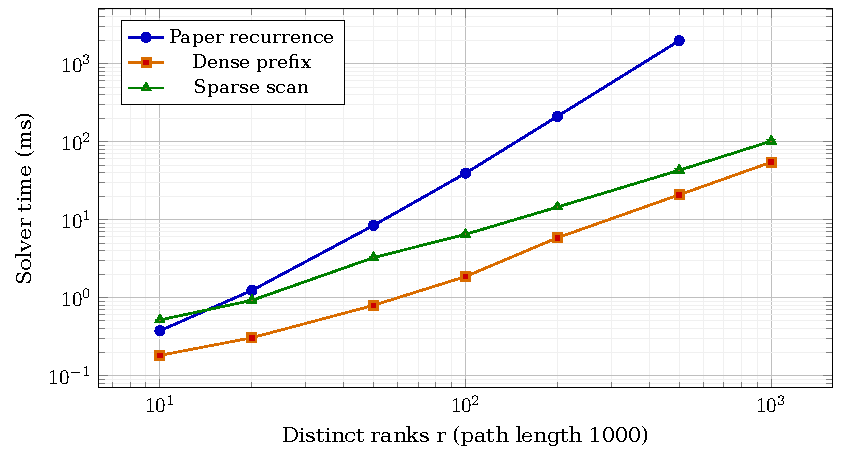
\includegraphics[width=0.94\textwidth]{../results/figures/forest-scaling.pdf}
\caption{Forest dài 1000 cạnh: median và IQR theo compressed $r$. Các điểm timeout của baseline không được vẽ thành giá trị hữu hạn.}
\label{fig:forest-repeated}
\end{figure}

Trong grid thưa ban đầu, một nhãn trồng chung trên mỗi cạnh cho đáp án không rỗng, nhưng tại cardinality một thì $r$ cũng nén còn một. Follow-up density control khắc phục: thêm một cạnh lá ngoài đường $s$--$z$ mang tất cả 1000 hạng. Nhờ vậy $r=1000$ cố định, đường có 1000 cạnh và thay đổi riêng cardinality nhãn trên đường. Cạnh lá không tạo thêm đường đi đơn giữa hai terminal.

\begin{table}[htbp]
\centering
\small
\setlength{\tabcolsep}{4pt}
\caption{Kiểm soát mật độ: đường dài 1000 cạnh, compressed rank cố định 1000.}
\label{tab:density-control}
\begin{tabular}{lrrrrr}
\toprule
Nhãn/cạnh $d$ & $r$ & Paper ms & Dense ms & Sparse ms & Dense/Sparse \\
\midrule
1 & 1000 & 6.94 & 3.33 & 0.228 & 14.6 \\
4 & 1000 & 10.9 & 3.38 & 0.338 & 10 \\
16 & 1000 & 28.9 & 3.69 & 0.905 & 4.08 \\
100 & 1000 & 189 & 6.98 & 6.64 & 1.05 \\
1000 & 1000 & T/O & 64.9 & 119 & 0.545 \\
\bottomrule
\end{tabular}
\end{table}

\begin{figure}[htbp]
\centering
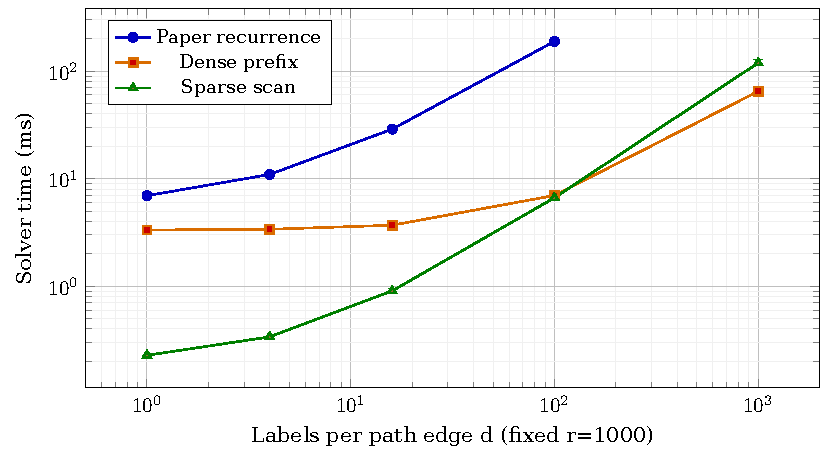
\includegraphics[width=0.94\textwidth]{../results/figures/density-control.pdf}
\caption{Giữ compressed $r=1000$ và chiều dài đường cố định, thay đổi số nhãn trên cạnh đường đi.}
\label{fig:density-control}
\end{figure}

H2 được đánh giá bằng phép đo kiểm soát này thay vì chỉ lấy graph có timestamp số lớn. Khi nhãn dày, mảng prefix có locality tốt hơn và có thể nhanh hơn sparse scan; khi nhãn ít, sparse solver tránh quét miền hạng trống. Vì các solver cùng kiểm tra cấu trúc và tra map, chi phí cố định giới hạn tỷ số tại cell nhỏ.

\FloatBarrier
\section{TTSP: ma trận so với sự kiện}

Mọi cell trong grid $k\in\{1,2,4,8,16,32,64,128,256\}$ và $r\in\{2,4,8,16,32\}$ đều được so đáp án với $2^k\binom{r+2k-1}{2k}$ bằng số nguyên Python; cả hai solver hoàn thành bảy lần đo trên toàn bộ 45 cell. Các cell strict dùng $2^k\binom{r}{2k}$. Đây là kiểm tra oracle trên toàn grid, không chỉ các trường hợp brute force nhỏ.

\begin{table}[htbp]
\centering
\small
\setlength{\tabcolsep}{4pt}
\caption{TTSP: median thời gian và maximum peak RSS qua các lần đo; skip là giới hạn ngân sách.}
\label{tab:ttsp-repeated}
\begin{tabular}{lrrrrrr}
\toprule
$k$ & $r$ thật & Matrix ms & Events ms & M/E & RSS M/E MiB & Bit \\
\midrule
1 & 32 & 0.736 & 0.0249 & 29.6 & 4.12/3.85 & 11 \\
16 & 32 & 18.5 & 0.393 & 47.2 & 9.2/4.09 & 76 \\
64 & 32 & 79 & 1.6 & 49.2 & 25.4/4.8 & 174 \\
256 & 32 & 365 & 7.53 & 48.4 & 92.6/8.01 & 424 \\
32 & 128 & 1.71e+03 & 2.2 & 776 & 167/5.65 & 204 \\
1024 & 7082 & skip & 14.8 & -- & --/7.14 & 1029 \\
\bottomrule
\end{tabular}
\end{table}


Tại $k=256,r=32$, graph có 1024 cạnh tĩnh, 32768 cạnh thời gian và đáp án 424 bit. Median ma trận là \TTSPMatrixTime{} ms; sự kiện là \TTSPEventTime{} ms, tỷ số \TTSPSpeedup{} lần. Maximum peak RSS qua các mẫu lần lượt \TTSPMatrixRSS{} và \TTSPEventRSS{} MiB. Telemetry quét sự kiện ghi đúng một phép cộng cho mỗi cạnh thời gian, phù hợp với cận số học trong \cref{thm:ttsp-events}.

\begin{figure}[htbp]
\centering
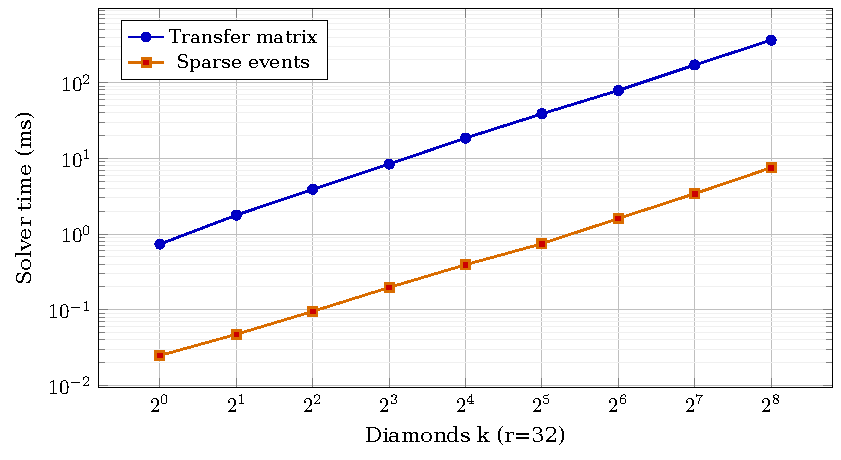
\includegraphics[width=0.94\textwidth]{../results/figures/ttsp-scaling.pdf}
\caption{TTSP tại $r=32$, median và IQR. Chi phí đọc/validate SP vẫn nằm trong thời gian solver.}
\label{fig:ttsp-events}
\end{figure}

Các graph thưa đến 1024 diamond dùng miền timestamp nominal 10000 và bốn nhãn/cạnh; bảng báo $r$ thực sự sau compression. Oracle vector SP bằng Python xác nhận count dù không thể liệt kê $2^{1024}$ tuyến. Ma trận vượt rank cap được ghi skip, không gán speedup hữu hạn cho một phép đo chưa chạy. Lõi sự kiện có cùng cơ sở đúng cho strict, nhưng benchmark strict là một tập riêng nhỏ hơn benchmark non-strict.

\FloatBarrier
\section{Treewidth: cận mới và miền thực dụng}

Trên 24 partial 2-tree cùng hoàn thành, trung bình nhân speedup DP mới so với DP cũ là \DPGeoSpeedup{} lần. Figure cố định $r=4$ và graph replicate 0 theo $n$; các seed khác nhau được nhận dạng trong raw CSV, nên không nhầm đây là cùng một graph được tăng dần đỉnh.

\begin{figure}[htbp]
\centering
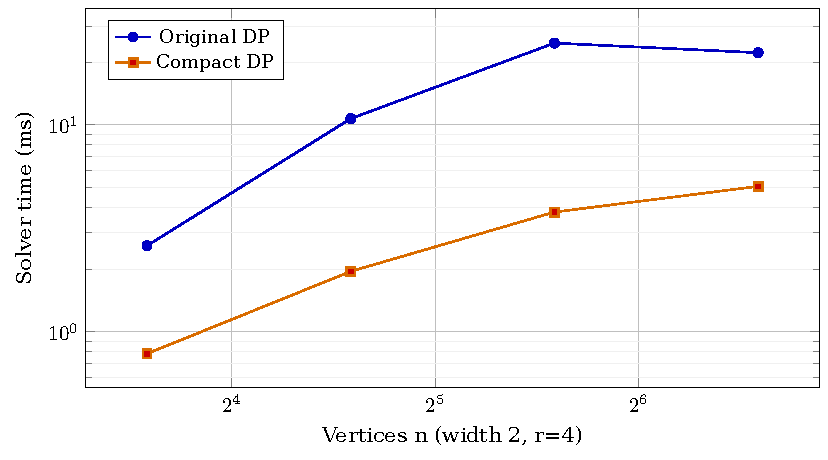
\includegraphics[width=0.94\textwidth]{../results/figures/partial2-scaling.pdf}
\caption{Partial 2-tree với terminal tùy ý: DP ban đầu và DP compact.}
\label{fig:partial2-scaling}
\end{figure}

\begin{table}[htbp]
\centering
\small
\setlength{\tabcolsep}{4pt}
\caption{Độ nhạy theo width tại n=12, r=8; mỗi width dùng một seed cố định.}
\label{tab:width-sensitivity}
\begin{tabular}{lrrrr}
\toprule
$w$ & Brute ms & DP cũ ms & DP mới ms & Trạng thái mới \\
\midrule
1 & 0.00117 & 0.429 & 0.171 & 272 \\
2 & 0.0312 & 17.5 & 3.07 & 4.83e+03 \\
3 & 1.49 & 272 & 15 & 1.8e+04 \\
4 & 12.7 & T/O & 381 & 4.32e+05 \\
\bottomrule
\end{tabular}
\end{table}

\begin{figure}[htbp]
\centering
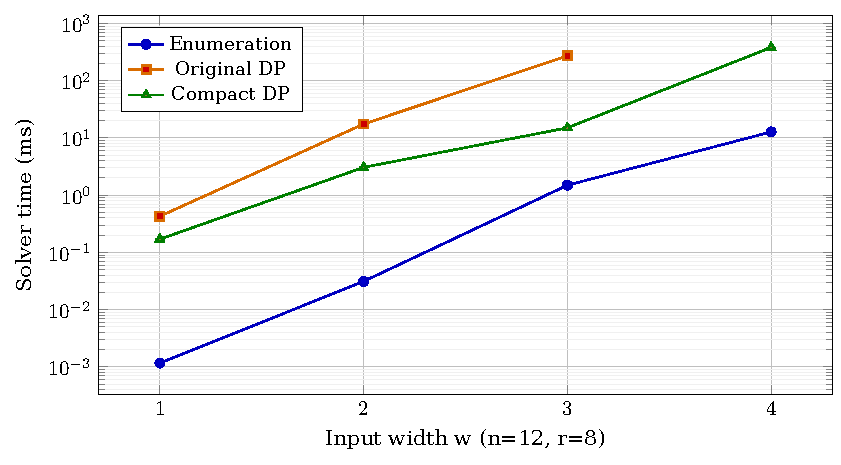
\includegraphics[width=0.94\textwidth]{../results/figures/width-scaling.pdf}
\caption{Độ nhạy với width tại $n=12,r=8$. Enumeration được đo và không bị loại khi thắng ở miền nhỏ.}
\label{fig:width-sensitivity}
\end{figure}

Ở $n=12$, enumeration có thể thắng DP vì chi phí tổ chức trạng thái lớn hơn lượng đường phải liệt kê. Khi width tăng, số trạng thái và chi phí join tăng mạnh dù số đỉnh không đổi. Điều này phù hợp với XP: cận đa thức khi width cố định không đồng nghĩa mọi width đều thực dụng. Bảng timeout thể hiện giới hạn đo được thay vì dùng chúng để khẳng định FPT.

\begin{table}[htbp]
\centering
\small
\setlength{\tabcolsep}{4pt}
\caption{Ablation trên ba partial 2-tree: GM của median thời gian; median telemetry theo instance.}
\label{tab:ablation}
\begin{tabular}{lrrrr}
\toprule
Cấu hình & Median-GM ms & States & Peak live & Join thử/có thể \\
\midrule
DP cũ & 32.4 & 18\,785 & 18\,785 & 100\% \\
Đầy đủ & 5.46 & 6\,801 & 854 & 40.1\% \\
Bỏ compact & 11.8 & 11\,324 & 2\,197 & 37.5\% \\
Bỏ prune và compact & 24.9 & 18\,785 & 4\,957 & 34.6\% \\
Bỏ index join & 6.49 & 6\,801 & 854 & 100\% \\
Giữ bảng con & 5.73 & 6\,801 & 6\,801 & 40.1\% \\
\bottomrule
\end{tabular}
\end{table}


Tỷ số trung bình nhân giữa baseline và bản đầy đủ trên ba instance ablation là \AblationCombinedSpeedup{} lần. \code{no-compact} giữ pruning nhưng lưu timestamp terminal; \code{no-prune} cũng phải tắt compaction vì quotient dựa trên ràng buộc terminal. Muốn tách riêng pruning, so \code{no-prune} với \code{no-compact}; muốn tách compaction, so \code{no-compact} với bản đầy đủ. \code{no-index} và \code{no-release} lần lượt đổi một yếu tố. Peak live states đo vòng đời bảng, còn RSS đo toàn address space, nên hai đại lượng không được đồng nhất.

\FloatBarrier
\section{Enumeration crossover và ladder hàm mũ}

\begin{table}[htbp]
\centering
\small
\setlength{\tabcolsep}{4pt}
\caption{Enumeration crossover tại width 2, r=4; các seed khác nhau được báo cáo đầy đủ.}
\label{tab:enumeration-crossover}
\begin{tabular}{lrr}
\toprule
$n$ & Enumeration ms & Treewidth ms \\
\midrule
12 & 0.0242 & 0.751 \\
24 & 1.07 & 2.03 \\
48 & 1.23 & 4.01 \\
96 & 98.7 & 5.09 \\
\bottomrule
\end{tabular}
\end{table}


Không tuyên bố DP luôn nhanh hơn enumeration: ở các graph ngẫu nhiên nhỏ, baseline đơn giản có thể thắng. Crossover còn phụ thuộc query, nhãn và topology. Để tách tác động số tuyến, ladder hai hàng tạo một họ width hai với oracle độc lập và số tuyến tăng hàm mũ.

\begin{proposition}[Oracle ladder]
Ladder $c$ cột, nguồn top-left và đích bottom-right, có $2^{c-1}$ đường đi tĩnh đơn. Nếu mỗi cạnh hoạt động ở mọi hạng $1..r$, số non-strict temporal paths là
\[
 \sum_{\substack{1\le q\le c\\q\ \mathrm{lẻ}}}
 \binom cq\binom{r+c+q-2}{c-1+q}.
\]
Với strict, thay thừa số thứ hai bằng $\binom r{c-1+q}$.
\end{proposition}

\begin{proof}
Mỗi cut giữa hai cột có đúng hai cạnh ngang. Đường đơn nối nguồn bên trái với đích bên phải phải vượt cut số lần lẻ và dùng mỗi cạnh tối đa một lần; vì thế vượt đúng một lần, theo hướng trái sang phải. Đường chọn một tập $q$ rung tại các cột; cần $q$ lẻ để đổi từ hàng trên sang hàng dưới. Mỗi tập rung lẻ xác định duy nhất một đường đơn dài $c-1+q$. Có $\binom cq$ tuyến tương ứng; áp dụng oracle nhãn cho từng độ dài. Tổng số tập con lẻ là $2^{c-1}$.
\end{proof}

Ladder từ ba cột không phải cactus; các cạnh có thể thuộc nhiều chu trình. Hai đường đơn của cùng truy vấn có thể dùng một rung theo hai hướng trái ngược, nên không áp dụng định hướng TTSP cực--cực sẵn có. Đây là stress case cho thuật toán SP với đầu cuối tùy ý, không chỉ cho solver cactus.

\begin{table}[htbp]
\centering
\small
\setlength{\tabcolsep}{4pt}
\caption{Ladder width hai với r=4 và truy vấn top-left/bottom-right; oracle đóng cho mọi cell.}
\label{tab:ladder}
\begin{tabular}{lrrrr}
\toprule
Cột $c$ & Tuyến tĩnh & Brute ms & DP cũ ms & DP mới ms \\
\midrule
4 & $2^{3}$ & 0.00737 & 1.3 & 0.303 \\
8 & $2^{7}$ & 0.25 & 3.73 & 0.876 \\
12 & $2^{11}$ & 6.25 & 5.76 & 1.47 \\
16 & $2^{15}$ & 138 & 9.07 & 2.04 \\
24 & $2^{23}$ & T/O & 14.2 & 3.16 \\
32 & $2^{31}$ & T/O & 19.4 & 4.66 \\
64 & $2^{63}$ & T/O & 40.6 & 9.38 \\
\bottomrule
\end{tabular}
\end{table}

\begin{figure}[htbp]
\centering
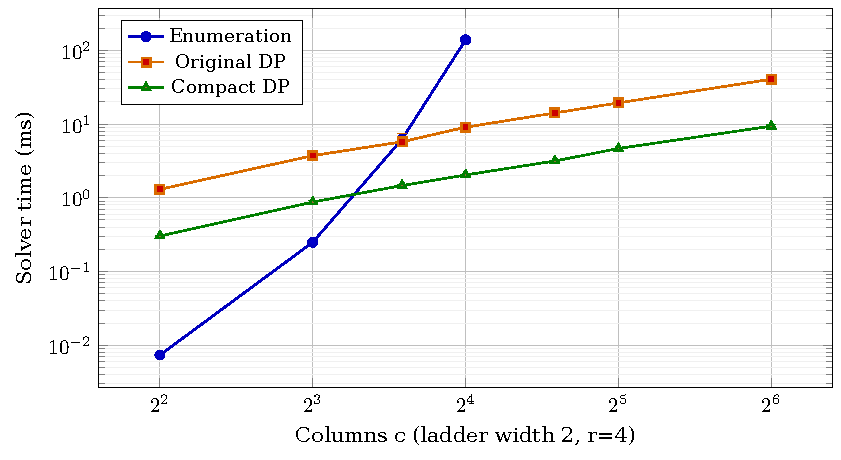
\includegraphics[width=0.94\textwidth]{../results/figures/ladder-scaling.pdf}
\caption{Ladder width hai tại $r=4$. Median/IQR của enumeration và hai phiên bản DP; cell timeout được giữ trong bảng.}
\label{fig:ladder-scaling}
\end{figure}

Ladder 64 cột có $2^{63}$ tuyến tĩnh. DP trả count chính xác so với công thức, trong khi enumeration vượt timeout. Điều này kiểm chứng khả năng nén nghiệm mà các instance rất nhỏ dùng làm oracle không thể thể hiện.

\FloatBarrier
\section{Cactus với truy vấn nội bộ}

Chọn hai đỉnh giữa ở diamond đầu và cuối của chuỗi $k\ge2$ diamond. Mỗi block đầu/cuối có hai cung dài một hoặc ba; các block giữa đóng góp hai lựa chọn dài hai. Oracle là
\[
2^{k-2}\left[
 \binom{r+2k-3}{2k-2}+2\binom{r+2k-1}{2k}+\binom{r+2k+1}{2k+2}
\right].
\]
Query không trùng cực gốc của biểu thức ban đầu. Cactus solver tự xây route theo query, không nhận decomposition ngoài. Trung bình nhân speedup so với generic treewidth DP trên tám cell là \CactusGeoSpeedup{} lần; đây là so sánh nội bộ giữa hai thuật toán của khóa luận.

\begin{table}[htbp]
\centering
\small
\setlength{\tabcolsep}{4pt}
\caption{Cactus với đầu cuối nội bộ tùy ý; toàn bộ đáp án đối chiếu công thức độc lập.}
\label{tab:cactus-repeated}
\begin{tabular}{lrrr}
\toprule
$k$ & Cactus ms & Treewidth ms & DP/Cactus \\
\midrule
4 & 0.0208 & 2 & 96.1 \\
16 & 0.0989 & 11.8 & 119 \\
64 & 0.354 & 51.3 & 145 \\
256 & 1.53 & 218 & 143 \\
\bottomrule
\end{tabular}
\end{table}

\begin{figure}[htbp]
\centering
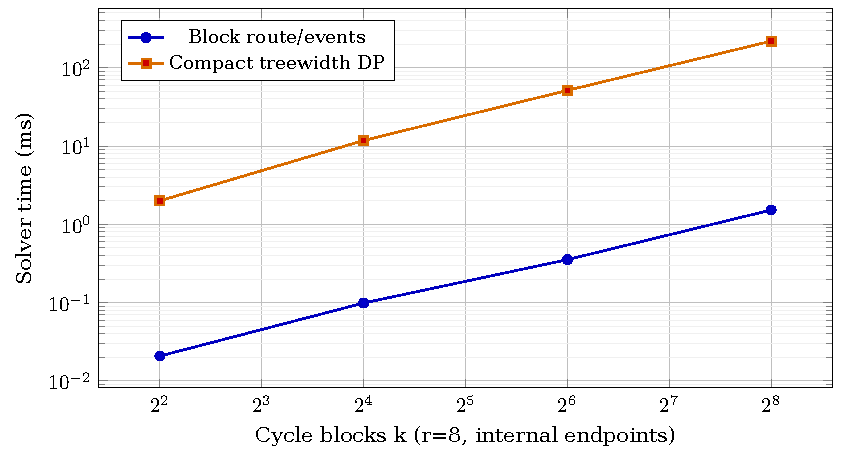
\includegraphics[width=0.94\textwidth]{../results/figures/cactus-scaling.pdf}
\caption{Cactus có đầu cuối nội bộ: block route/sự kiện và DP treewidth tổng quát.}
\label{fig:cactus-scaling}
\end{figure}

\FloatBarrier
\section{Censoring và giới hạn}

\begin{table}[htbp]
\centering
\small
\setlength{\tabcolsep}{4pt}
\caption{Mọi solver/cell không hoàn thành; không bị loại khỏi báo cáo.}
\label{tab:censored}
\begin{tabular}{llll}
\toprule
Họ & Instance & Solver & Trạng thái \\
\midrule
forest\_dense & L500-r1000 & forest-paper & timeout \\
forest\_dense & L1000-r1000 & forest-paper & timeout \\
forest\_sparse & L1000-r1000-d1000 & forest-paper & timeout \\
forest\_density\_control & L1000-r1000-d1000 & forest-paper & timeout \\
ttsp\_extra & k64-r128-strict0 & ttsp-transfer & timeout \\
ttsp\_sparse & k64-r1000-d4 & ttsp-transfer & skipped\_budget \\
ttsp\_sparse & k256-r10000-d4 & ttsp-transfer & skipped\_budget \\
ttsp\_sparse & k1024-r10000-d4 & ttsp-transfer & skipped\_budget \\
width & w4-n12-r8 & tw-dp-baseline & timeout \\
ladder & c24-r2 & brute & timeout \\
ladder & c24-r4 & brute & timeout \\
ladder & c24-r8 & brute & timeout \\
ladder & c32-r2 & brute & timeout \\
ladder & c32-r4 & brute & timeout \\
ladder & c32-r8 & brute & timeout \\
ladder & c64-r2 & brute & timeout \\
ladder & c64-r4 & brute & timeout \\
ladder & c64-r8 & brute & timeout \\
\bottomrule
\end{tabular}
\end{table}


T/O là subprocess không kết thúc trong ba giây; skip là quyết định ngân sách trước khi chạy. Không thay timeout bằng đúng ba giây để tính median, không loại chúng khỏi bảng phạm vi, và không lấy ratio của hai loại timing khác nhau. CSV/summary đầy đủ là nguồn số liệu chính; các bảng trong chương chỉ chọn cell đại diện theo kích thước đã mô tả.

\paragraph{Nội tại.} BigInt tự cài có rủi ro, được kiểm tra bằng số nguyên Python, oracle đóng và sanitizer. Bảy mẫu và pinning giảm nhiễu nhưng không khóa tần số hay tạo máy benchmark riêng. RSS không đo chính xác heap được dùng cho DP. Lõi $\bigO(M)$ theo số phép cộng vẫn có chi phí tăng với số bit.

\paragraph{Ngoại tại.} Dữ liệu chính là synthetic theo theorem và Graph Atlas cho correctness. Không có mạng thời gian thực trong chiến dịch này; graph thực có width cao không tự thuộc miền thuật toán. Vì vậy không suy rộng tốc độ SP sang mọi mạng xã hội/giao thông.

\paragraph{Kết luận.} Audit lớn không chứng minh đúng thay cho chứng minh; chưa vét cạn $n=5,r=2$. Tham số và seed được ghi rõ, nhưng vài graph mỗi cell không đại diện cho mọi phân phối. Geometric mean chỉ dùng cell cùng hoàn thành và không diễn tả riêng tỷ lệ timeout; hai chỉ số được báo song song.

\paragraph{Tính mới.} Rà soát cập nhật đọc thêm các nguồn 2025--2026, nhưng chưa có kết luận phản biện độc lập về ưu tiên công bố. Khóa luận đã đưa ra định lý, mã và bằng chứng kiểm tra; việc xác lập kết quả học thuật cuối cùng là bước thẩm định riêng.

\chapter{Kết luận và hướng phát triển}
\label{chap:conclusion}

\section{Kết quả thuật toán}

Khóa luận chuyển câu hỏi đếm đường đi thời gian trên cấu trúc hẹp thành các thuật toán và cận kiểm tra được. Trên rừng, đánh giá lại cùng truy hồi bằng tổng tiền tố hoặc hai con trỏ giảm chi phí theo số hạng và số nhãn thực sự. Đây là cải tiến của thuật toán trên cùng miền với paper, không phải lời giải cho graph tổng quát.

Trên TTSP cực--cực, ma trận truyền cung cấp một đại số đúng nhưng dư thông tin cho một truy vấn. Song ánh với DAG cho phép thay phép nhân ma trận bằng quét sự kiện, thực hiện đúng một phép cộng mỗi time-edge sau tiền xử lý. Cactus dùng route block--cut để mở rộng miền truy vấn mà vẫn giữ một định hướng tương đương. Wheatstone và ladder làm rõ vì sao hướng này không tự bao phủ mọi query SP.

DP treewidth giải miền tổng quát hơn bằng trạng thái thời gian cục bộ và phân hoạch liên thông. Đẳng thức $\beta(F_1\cup F_2)=\beta(J)$ chứng minh điều kiện join, kể cả multiedge trong incidence graph. Terminal quotient chỉ giữ trạng thái đã dùng cạnh, giảm exponent trạng thái theo $r$ từ $w+3$ xuống $w+1$. Cận mới $N(r+1)^{2w+2}2^{\bigO(w\log w)}$ cho width hai là $\bigO(N(r+1)^6)$. Thay so sánh và tie ordering cho strict giữ nguyên cấu trúc chứng minh trên các lớp này.

\section{Trả lời câu hỏi nghiên cứu}

\paragraph{RQ1.} Có cải tiến cận đánh giá forest: từ $\bigO(|P|r^2)$ của bản truy hồi trực tiếp sau compression xuống $\bigO(|P|r)$ hoặc $\bigO(|P|+M_P)$ theo số phép toán số học. Trên \ForestPairedCells{} cell dày cùng hoàn thành, trung bình nhân speedup là \ForestGeoSpeedup{} lần; density control giữ $r$ cố định xác nhận lợi ích của nhãn thưa.

\paragraph{RQ2.} TTSP cực--cực có lõi quét $\bigO(n+m+M+r)$ sau định hướng/nén hạng. Tại 256 diamond và 32 hạng, median sự kiện \TTSPEventTime{} ms so với ma trận \TTSPMatrixTime{} ms. Chi phí input, structural validation và độ dài bit vẫn được nêu riêng.

\paragraph{RQ3.} DP tường minh thuộc XP theo treewidth. Width hai cho thuật toán đa thức với terminal tùy ý, kể cả các graph như ladder không được giải bằng một định hướng TTSP theo query. Không kết luận FPT chỉ theo treewidth hoặc giải \#P-hard counting trong graph bất kỳ.

\paragraph{RQ4.} Cài đặt có \AuditComparisons{} đối chiếu mới không sai lệch và \BenchCases{} cấu hình đo lặp. Oracle Python/time-edge enumeration, công thức đóng và metamorphic tests kiểm tra những cơ chế khác nhau. Telemetry ablation giúp phân biệt cải tiến cận trạng thái, số cặp join và thời gian sống bảng. Benchmark lưu cả \BenchTimeouts{} timeout và \BenchSkips{} budget skip.

\section{Mức độ đóng góp so với paper}

So với kết quả forest của paper, khóa luận cải thiện đánh giá truy hồi và cung cấp số liệu thực thi. So với giả thuyết series--parallel, khóa luận đưa ra một lời giải đa thức tường minh trong bản thảo, cài đặt và các test có cặp đầu cuối tùy ý. TTSP sự kiện và cactus là thuật toán chuyên biệt có cận tốt hơn baseline ma trận của chính dự án. Strict mở rộng các định lý đang xét, không tự chuyển toàn bộ hardness/approximation results của paper.

Các thành phần như prefix sum, Tarjan, topological sort và partition DP là chuẩn. Đóng góp cần được đánh giá ở tính đúng của cách kết hợp, trạng thái tối giản, phạm vi định lý và bằng chứng tái lập. Rà soát đã bổ sung nguồn 2025--2026 nhưng chưa có kết luận độc lập về ưu tiên công bố. Cách phát biểu phù hợp là ``đề xuất và chứng minh trong khóa luận một lời giải đa thức cho trường hợp SP'', với tính mới quốc tế là đối tượng thẩm định tiếp theo.

\section{Hạn chế còn lại}

XP có số mũ phụ thuộc width và cận thô còn lớn; độ nhạy thực nghiệm width bốn đã cho thấy giới hạn. Join indexing không thay đổi exponent xấu nhất. Cận bộ nhớ sau giải phóng bảng phụ thuộc frontier/chiều cao decomposition; chưa tối ưu lịch đánh giá và packing toàn bộ trạng thái.

Vét cạn toàn bộ $n=5,r=2$ chưa hoàn thành. Chiến dịch có dữ liệu tổng hợp và Atlas, chưa có mạng thời gian thực. Bảy lượt đo không loại hết DVFS/nhiễu; RSS gồm parsing và allocator. Phân rã width không quá hai được hỗ trợ, nhưng width cao nhận TD ngoài; không giải bài toán tìm treewidth tối ưu tổng quát.

\section{Các hướng nghiên cứu tiếp theo}

Ưu tiên lý thuyết là phản biện độc lập các định lý, đặc biệt quotient terminal, tính đầy đủ tại forget và join incidence. Tiếp theo, tìm DP riêng cho query SP tùy ý có exponent nhỏ hơn sáu; hoặc khai thác nhiều query dùng chung preprocessing để giảm chi phí lặp. Nghiên cứu ranh giới FPT/XP theo treewidth đòi hỏi kết quả riêng, không suy từ tối ưu engineering hiện tại.

Về thực nghiệm, mở rộng vét cạn bằng runner checkpoint và chia miền cấu hình; đo trên máy kiểm soát tần số với nhiều seed độc lập. Có thể thêm dữ liệu thực sau khi định nghĩa rõ phép trích subgraph width thấp và tỷ lệ giữ lại. Những kết quả trên subgraph phải được báo đúng phạm vi, không như lời giải trên toàn bộ mạng.

Về phần mềm, dùng thư viện số nguyên lớn đã được kiểm chứng rộng rãi để đối chiếu thêm, tối ưu parser/lookup, lịch giải phóng bảng và stack đánh giá TD. Các bước này có thể cải thiện end-to-end performance sau khi lõi đếm đã nhanh, và phải đo lại bằng đúng protocol cùng source hash.


\appendix
\chapter{Định dạng dữ liệu và decomposition}

\section{Temporal graph}

Ví dụ:
\begin{lstlisting}[numbers=none]
p 3 4 0 2
0 1 1
0 1 2
1 2 2
1 2 3
\end{lstlisting}
Header lần lượt là số đỉnh, số dòng temporal edge, nguồn và đích. Đỉnh đánh số từ $0$. Cài đặt nhận timestamp là số nguyên có dấu 64 bit, kể cả âm, rồi nén hạng khi đọc. Không dùng độ lớn timestamp làm kích thước mảng.

\section{TTSP expression}

File SP dùng node ID và root:
\begin{lstlisting}[numbers=none]
sp 7 6
0 edge 0 1
1 edge 1 3
2 series 0 1
3 edge 0 2
4 edge 2 3
5 series 3 4
6 parallel 2 5
\end{lstlisting}
Node phải tạo thành DAG biểu thức thực tế là cây; cực có thứ tự của hai con series phải gặp nhau và hai con parallel phải có cùng cực.

\section{Nice tree decomposition}

Header có số node, root và width của decomposition đầu vào trước chuẩn hóa. Các dạng dòng:
\begin{lstlisting}[numbers=none]
ntd NODE_COUNT ROOT WIDTH
ID leaf BAG_SIZE BAG...
ID introduce-v CHILD V BAG_SIZE BAG...
ID introduce-e CHILD U V BAG_SIZE BAG...
ID forget-v CHILD V BAG_SIZE BAG...
ID join LEFT RIGHT BAG_SIZE BAG...
\end{lstlisting}
Cài đặt yêu cầu $s,z$ trong mọi bag và root đúng bằng $\{s,z\}$. Mỗi static edge phải xuất hiện trong đúng một node \code{introduce-e}.

\section{Schema kết quả}

CSV mới chứa family, instance ID, seed, replicate, solver/ablation, status, $n$, số cạnh tĩnh/thời gian, $r$ thật và nominal, cận trên width phân rã, terminal, strict flag, đáp án, bit length, solver wall/CPU time, parse/subprocess time, batch repeats, RSS, số trạng thái và join pairs. Hash input, decomposition, đáp án, source và binary nhận dạng artifact; compiler, flags, machine và controller/generator hash được lưu trong metadata JSON đi kèm. Không phụ thuộc vào một Git commit chưa tồn tại để xác định bản source. Trường width không phải khẳng định width tối tiểu sau khi xóa cạnh.

\chapter{Hướng dẫn tái lập}

\section{Build}

Yêu cầu GCC/Clang hỗ trợ C++20 và Python 3.10 trở lên.
\begin{lstlisting}[language=bash,numbers=none]
bash scripts/build.sh
\end{lstlisting}
Trên máy có CMake backend:
\begin{lstlisting}[language=bash,numbers=none]
cmake -S . -B build -DCMAKE_BUILD_TYPE=Release -DTPCOUNT_NATIVE=ON
cmake --build build -j
ctest --test-dir build --output-on-failure
\end{lstlisting}

\section{Chiến dịch nghiên cứu mới}

\begin{lstlisting}[language=bash,numbers=none]
# Kiem chung vet can, Python DFS, Atlas, metamorphic
python3 python/research_audit.py

# 169 instance, warm-up + 7 measured batches
python3 python/research_benchmark.py

# 21 ladder cells, giao thuc rieng, cung binary
python3 python/ladder_benchmark.py

# Bang, hinh, macro LaTeX tu hai CSV cuoi
python3 python/research_aggregate.py
\end{lstlisting}

Pipeline đầy đủ nằm trong \nolinkurl{scripts/research_pipeline.sh}, chạy bằng Bash. Không chạy audit, compile hoặc tải nặng đồng thời với benchmark. Script ghim một CPU trong affinity cho phép nhưng không khóa xung CPU; vì vậy không kỳ vọng tái lập chính xác từng microsecond trên máy khác. Mỗi cell thành công phải đủ bảy mẫu; timeout và giới hạn ngân sách được giữ nguyên. Các tệp metadata nhận dạng binary, source, controller, generator và cấu hình đo.

\nolinkurl{results/research_benchmark.csv} và \nolinkurl{results/research_ladder.csv} là hai CSV nguồn cuối. \nolinkurl{results/research_benchmark_summary.csv} chứa median, quartile, IQR, RSS và telemetry. Bảng và macro trong \code{thesis/generated/} do script sinh, không sửa số bằng tay. Dữ liệu lịch sử, pilot và RSS trước sửa lỗi nằm ngoài aggregate cuối.

Audit vét cạn là $n\le4,r=2$ và $n=5,r=1$, không phải toàn bộ $n=5,r=2$. Graph Atlas dùng bản gzip được giữ trong \code{benchmarks/data/}, với URL, giấy phép và SHA-256 trong README đi kèm. Số \AuditComparisons{} là tổng đối chiếu solver, không phải số graph khác nhau.

\section{Chạy solver và nhận dạng width hai}

\begin{lstlisting}[language=bash,numbers=none]
build/tpcount count --solver ttsp-events INSTANCE.tg --decomp INSTANCE.sp
build/tpcount count --solver cactus INSTANCE.tg
python3 python/decompose.py INSTANCE.tg INSTANCE.ntd
build/tpcount verify --solver tw-dp INSTANCE.tg --td INSTANCE.ntd --reference cartesian
build/tpcount count --solver tw-dp INSTANCE.tg --td INSTANCE.ntd --strict --repeat 20
\end{lstlisting}
Với graph lớn, không dùng DFS tham chiếu nếu số tuyến/nhãn có thể tăng hàm mũ; dùng oracle đóng hoặc oracle biểu thức SP độc lập khi phù hợp. Định dạng decomposition được mô tả trong repository. Nice hóa bằng Python hiện dùng đệ quy, nên pipeline nhận dạng không được quảng bá là bộ tiền xử lý tuyến tính chịu được mọi độ sâu.

\section{Biên dịch khóa luận}

Repository cung cấp script Tectonic:
\begin{lstlisting}[language=bash,numbers=none]
bash thesis/build_pdf.sh
python3 python/research_validate.py
\end{lstlisting}
Script tự biên dịch bảy hình vector PGFPlots trước bản thảo; cần Tectonic, font DejaVu/FreeMono, hoặc Nix có package tương ứng. Kết quả là \code{results/temporal\_path\_thesis.pdf}. Integrity validator kiểm tra đủ bảy mẫu riêng biệt, count/hash, thống kê summary, input và source/binary không đổi, audit digest, hình/PDF không cũ hơn source; kết quả ghi trong \nolinkurl{results/research_release_validation.json}. Trước khi nộp, thay các macro thông tin cá nhân ở đầu \code{thesis/main.tex}, cập nhật \code{CITATION.cff}, lưu phiên bản source rõ ràng, và chạy lại toàn bộ bảng/hình trên máy được mô tả trong khóa luận. Hoàn thành phản biện chứng minh và rà soát novelty độc lập, tuân thủ quy định công bố hỗ trợ AI của cơ sở đào tạo; không dùng benchmark để thay cho các bước này.

\chapter{Thẩm định chứng minh}

\begin{enumerate}[label=$\square$,leftmargin=1.2cm]
  \item Mô hình so sánh chính khớp bài báo 2025: thời gian $\le$; biến thể strict $<$ được ghi tách biệt, không trộn đáp án.
  \item Mỗi static edge được introduce đúng một lần và chỉ chọn tối đa một timestamp.
  \item Ràng buộc indegree/outdegree ngăn branching.
  \item Cycle test tại introduce-edge đúng.
  \item Đỉnh nonterminal được dùng phải là \textsc{Both} trước khi forget.
  \item Không thành phần nào biến mất khỏi separator.
  \item Incidence multigraph lemma dùng đồng nhất cycle rank $\beta(U)=\beta(J)$, bao gồm chu trình hai cạnh song song; không suy diễn từ closed walk sang cycle.
  \item Phân hoạch cha ở join là bao đóng đúng của hai quan hệ con.
  \item Root loại mọi thành phần dư và buộc đúng một đường $s$--$z$.
  \item Hướng của đường bắt buộc từ $s$ tới $z$.
  \item Bất đẳng thức cục bộ suy ra dãy nhãn không giảm, hoặc tăng nghiêm ngặt trong chế độ strict.
  \item Completeness sử dụng đúng tính liên thông của bag chứa một đỉnh.
  \item Không có double count do edge introduction duy nhất.
  \item Compact timestamp ở $s,z$ chỉ bật cùng terminal pruning; không có ràng buộc so thời gian tại hai terminal.
  \item State bound tính cả Bell partitions và chỉ $w+1$ nonterminal trong bag chuẩn hóa; cận width hai là $\bigO(N(r+1)^6)$ phép toán số học.
  \item Độ dài bit của số đếm là đa thức với $w$ cố định.
  \item Thuật ngữ TTSP, series--parallel và partial $2$-tree được phân biệt đúng.
  \item Định hướng TTSP giữ đúng mọi đường cực--cực; cactus giữ đúng mọi đường theo tuyến block--cut; không mở rộng lemma này sang Wheatstone tùy ý.
  \item Tie ordering của sự kiện incoming/outgoing đúng cho cả $\le$ và $<$; mỗi temporal edge sinh đúng một phép cộng.
  \item Parsing, validation, xây decomposition và chi phí bit được tách khỏi cận số phép toán; RSS đo đúng address space sau exec.
  \item Novelty claim đã được kiểm tra độc lập và cập nhật đến ngày nộp.
\end{enumerate}

Không đánh dấu một mục chỉ dựa trên unit test. Checklist này dành cho giảng viên hướng dẫn hoặc phản biện độc lập đọc chứng minh và đối chiếu mã nguồn.

\chapter{Các điểm phản biện và cách kiểm tra}

\section{Đâu là phần cải tiến trực tiếp paper?}

Forest là miền đối chiếu trực tiếp: dùng cùng input, rank compression và số nguyên chính xác, đánh giá lại truy hồi đã công bố. Matrix và treewidth baseline là phiên bản nội bộ, không phải mã tác giả. Paper còn có hardness, approximation và các tham số khác; khóa luận không tuyên bố thay thế các kết quả đó.

\section{Tại sao không dùng temporal walks thay cho paths?}

Tam giác có mọi cạnh tại thời điểm một cho phép một walk đi quanh chu trình vô hạn lần theo quy ước non-strict. Số đường đi đơn giữa hai đỉnh vẫn hữu hạn. Vì vậy mô hình phải giữ điều kiện không lặp đỉnh; DAG orientation chỉ dùng khi có song ánh cấu trúc, còn DP treewidth giữ rừng, bậc và điều kiện terminal.

\section{Tại sao kiểm tra bậc chưa đủ ở join?}

Hai nhánh có thể chọn các đoạn $x\to a\to y$ và $y\to b\to x$ tại cùng thời điểm. Hợp có mỗi đỉnh bậc vào/ra một nhưng tạo chu trình. Hai block con đều chứa $x,y$, nên incidence graph có hai cạnh song song giữa cùng hai block. Cycle rank bằng một phát hiện chính xác cấu hình này. Các đỉnh $s,z$ khác có thể đang zero trong cùng bag; chỉ nhìn chữ ký bậc không đủ bảo toàn bất biến rừng.

\section{Có thể quên nhãn terminal vì sao?}

Tại $s$ không tồn tại cạnh vào cần so với cạnh ra, tại $z$ không tồn tại cạnh ra cần so với cạnh vào. Nhãn của cạnh kề vẫn lưu ở đầu nonterminal khi cần kiểm tra. Nếu không cấm incoming $s$/outgoing $z$, placeholder terminal có thể bị dùng sai như một timestamp; do đó code chỉ compact khi pruning được bật. Label của cạnh trực tiếp $s\to z$ tạo nhiều realization khác nhau và được cộng trong count, dù state của chúng giống nhau.

\section{Một thời điểm có đúng hai kết quả khác nhau không?}

Đường $s-u-z$ với cả hai cạnh tại thời điểm một có count non-strict bằng một và strict bằng không. Quét sự kiện incoming trước outgoing đếm được nghiệm bằng thời điểm; đảo nhóm loại nó. Chỉ đổi một dấu trong oracle mà không đổi tie ordering của solver sẽ tạo lỗi có thể phát hiện bởi test này.

\section{Tại sao width hai chưa phải FPT theo width?}

Đặt $w=2$ thì exponent theo $r$ là sáu, một hằng số. Khi $w$ là tham số thay đổi, exponent $2w+2$ cũng thay đổi; không có cận $f(w)L^c$ với $c$ độc lập khỏi $w$ từ công thức này. Vì thế phân loại là XP. Số nguyên có nhiều bit được xử lý với cận bit riêng và không phá tính đa thức với width cố định.

\section{Zero mismatch cho phép khẳng định điều gì?}

Nó xác nhận các cài đặt và oracle đồng ý trên đúng tập đã ghi nhận. Nó không cho xác suất đúng toàn cục 100\%, không xác nhận ưu tiên quốc tế và không biến một bộ randomized tests thành exhaustive campaign. Ngược lại, chứng minh đúng cần đủ bất biến, case analysis và tính duy nhất của lựa chọn cạnh; bản thảo cung cấp các lập luận đó để người khác phản biện.

\section{Tại sao số RSS trước và sau sửa khác nhau?}

Fork trước exec có thể đưa dấu đỉnh bộ nhớ của Python vào \code{ru\_maxrss}; một chương trình C++ nhỏ vì vậy bị báo bộ nhớ lớn dù đã thay address space. \code{VmHWM} trong \code{/proc/self/status} thuộc address space hiện tại. Dữ liệu cũ được lưu riêng, toàn bộ số liệu cuối được đo lại; thuật toán đếm không thay đổi. Đây cũng là lý do phải tách peak RSS khỏi số trạng thái đang sống.

\section{Người thực hiện cần tự bảo vệ được gì?}

Trước khi nộp, tác giả cần tự diễn giải định nghĩa nghiệm, tự làm một transition introduce/forget/join, giải thích phản ví dụ Wheatstone, tính một oracle nhỏ và tái lập một cell từ mã nguồn. Các công cụ hỗ trợ lập trình, rà soát và soạn thảo không thay thế việc tác giả hiểu và chịu trách nhiệm về chứng minh, số liệu và cách ghi nhận hỗ trợ theo quy định của cơ sở đào tạo.


\begin{thebibliography}{99}

\bibitem{enright2025}
J.~Enright, K.~Meeks, and H.~Molter,
``Counting Temporal Paths,''
\emph{Algorithmica}, vol.~87, pp.~736--782, 2025.
doi: \href{https://doi.org/10.1007/s00453-025-01301-3}{10.1007/s00453-025-01301-3}.

\bibitem{enright2023}
J.~Enright, K.~Meeks, and H.~Molter,
``Counting Temporal Paths,''
in \emph{40th International Symposium on Theoretical Aspects of Computer Science (STACS 2023)},
LIPIcs, vol.~254, Article~30, 2023.
doi: \href{https://doi.org/10.4230/LIPIcs.STACS.2023.30}{10.4230/LIPIcs.STACS.2023.30}.

\bibitem{courcelle2012}
B.~Courcelle and J.~Engelfriet,
\emph{Graph Structure and Monadic Second-Order Logic: A Language-Theoretic Approach}.
Cambridge University Press, 2012.

\bibitem{eppstein1992}
D.~Eppstein,
``Parallel recognition of series-parallel graphs,''
\emph{Information and Computation}, vol.~98, no.~1, pp.~41--55, 1992.

\bibitem{michail2016}
O.~Michail,
``An introduction to temporal graphs: An algorithmic perspective,''
\emph{Internet Mathematics}, vol.~12, no.~4, pp.~239--280, 2016.

\bibitem{holme2019}
P.~Holme and J.~Saramäki,
\emph{Temporal Network Theory}.
Springer, 2019.

\bibitem{kempe2002}
D.~Kempe, J.~Kleinberg, and A.~Kumar,
``Connectivity and inference problems for temporal networks,''
\emph{Journal of Computer and System Sciences}, vol.~64, no.~4, pp.~820--842, 2002.

\bibitem{buss2024}
S.~Buß, H.~Molter, R.~Niedermeier, and M.~Rymar,
``Algorithmic aspects of temporal betweenness,''
\emph{Network Science}, vol.~12, no.~2, pp.~160--188, 2024.

\bibitem{casteigts2021}
A.~Casteigts, A.-S.~Himmel, H.~Molter, and P.~Zschoche,
``Finding temporal paths under waiting time constraints,''
\emph{Algorithmica}, vol.~83, no.~9, pp.~2754--2802, 2021.

\bibitem{valiant1979}
L.~G.~Valiant,
``The complexity of enumeration and reliability problems,''
\emph{SIAM Journal on Computing}, vol.~8, no.~3, pp.~410--421, 1979.

\bibitem{doering2026}
M.~Döring, J.~Enright, L.~Larios-Jones, and G.~Skretas,
``FO and MSO Model Checking on Temporal Graphs,''
in \emph{SAND 2026}, LIPIcs, vol.~373, Article~9, 2026.
doi: \href{https://doi.org/10.4230/LIPIcs.SAND.2026.9}{10.4230/LIPIcs.SAND.2026.9}.

\bibitem{enright2026}
J.~Enright, S.~D.~Hand, L.~Larios-Jones, and K.~Meeks,
``Families of Tractable Problems with Respect to Vertex-Interval-Membership Width and Its Generalisations,''
in \emph{SAND 2026}, LIPIcs, vol.~373, Article~4, 2026.
doi: \href{https://doi.org/10.4230/LIPIcs.SAND.2026.4}{10.4230/LIPIcs.SAND.2026.4}.

\bibitem{tang2025}
Z.~Tang, Y.~Wu, X.~Zai, C.~Chen, X.~Wang, and Y.~Zhang,
``Efficient Temporal Simple Path Graph Generation,''
arXiv:2507.10017, 2025.
\url{https://arxiv.org/abs/2507.10017}.

\bibitem{atlas1998}
R.~C.~Read and R.~J.~Wilson,
\emph{An Atlas of Graphs}. Oxford University Press, 1998.
Dataset distributed with NetworkX 3.5:
\url{https://networkx.org/documentation/stable/reference/generated/networkx.generators.atlas.graph_atlas_g.html}.

\end{thebibliography}

\end{document}
